%%%%%%%%%%%%%%%%%%%%%%%%%%%%%%%%%%%%%%%%%
% The Legrand Orange Book
% LaTeX Template
% Version 2.1.1 (14/2/16)
%
% This template has been downloaded from:
% http://www.LaTeXTemplates.com
%
% Original author:
% Mathias Legrand (legrand.mathias@gmail.com) with modifications by:
% Vel (vel@latextemplates.com)
%
% License:
% CC BY-NC-SA 3.0 (http://creativecommons.org/licenses/by-nc-sa/3.0/)
%
% Compiling this template:
% This template uses biber for its bibliography and makeindex for its index.
% When you first open the template, compile it from the command line with the
% commands below to make sure your LaTeX distribution is configured correctly:
%
% 1) pdflatex main
% 2) makeindex main.idx -s StyleInd.ist
% 3) biber main
% 4) pdflatex main x 2
%
% After this, when you wish to update the bibliography/index use the appropriate
% command above and make sure to compile with pdflatex several times
% afterwards to propagate your changes to the document.
%
% This template also uses a number of packages which may need to be
% updated to the newest versions for the template to compile. It is strongly
% recommended you update your LaTeX distribution if you have any
% compilation errors.
%
% Important note:
% Chapter heading images should have a 2:1 width:height ratio,
% e.g. 920px width and 460px height.
%
%%%%%%%%%%%%%%%%%%%%%%%%%%%%%%%%%%%%%%%%%

%----------------------------------------------------------------------------------------
%	PACKAGES AND OTHER DOCUMENT CONFIGURATIONS
%----------------------------------------------------------------------------------------

\documentclass[11pt,fleqn]{book} % Default font size and left-justified equations

%----------------------------------------------------------------------------------------

%%%%%%%%%%%%%%%%%%%%%%%%%%%%%%%%%%%%%%%%%
% The Legrand Orange Book
% Structural Definitions File
% Version 2.0 (9/2/15)
%
% Original author:
% Mathias Legrand (legrand.mathias@gmail.com) with modifications by:
% Vel (vel@latextemplates.com)
% 
% This file has been downloaded from:
% http://www.LaTeXTemplates.com
%
% License:
% CC BY-NC-SA 3.0 (http://creativecommons.org/licenses/by-nc-sa/3.0/)
%
%%%%%%%%%%%%%%%%%%%%%%%%%%%%%%%%%%%%%%%%%

%----------------------------------------------------------------------------------------
%	VARIOUS REQUIRED PACKAGES AND CONFIGURATIONS
%----------------------------------------------------------------------------------------

\usepackage[top=3cm,bottom=3cm,left=3cm,right=3cm,headsep=10pt,a4paper]{geometry} % Page margins

\usepackage{graphicx} % Required for including pictures
\graphicspath{{Pictures/}} % Specifies the directory where pictures are stored

\usepackage{lipsum} % Inserts dummy text

\usepackage{tikz} % Required for drawing custom shapes

\usepackage[english]{babel} % English language/hyphenation

\usepackage{enumitem} % Customize lists
\setlist{nolistsep} % Reduce spacing between bullet points and numbered lists

\usepackage{booktabs} % Required for nicer horizontal rules in tables

\usepackage{xcolor} % Required for specifying colors by name
\definecolor{ocre}{RGB}{243,102,25} % Define the orange color used for highlighting throughout the book

%----------------------------------------------------------------------------------------
%	FONTS
%----------------------------------------------------------------------------------------

\usepackage{avant} % Use the Avantgarde font for headings
%\usepackage{times} % Use the Times font for headings
\usepackage{mathptmx} % Use the Adobe Times Roman as the default text font together with math symbols from the Sym­bol, Chancery and Com­puter Modern fonts

\usepackage{microtype} % Slightly tweak font spacing for aesthetics
\usepackage[utf8]{inputenc} % Required for including letters with accents
\usepackage[T1]{fontenc} % Use 8-bit encoding that has 256 glyphs

%----------------------------------------------------------------------------------------
%	BIBLIOGRAPHY AND INDEX
%----------------------------------------------------------------------------------------

\usepackage{csquotes}
\usepackage[style=alphabetic,citestyle=numeric,sorting=nyt,sortcites=true,autopunct=true,autolang=hyphen,hyperref=true,abbreviate=false,backref=true,backend=biber,defernumbers=true]{biblatex}
\addbibresource{bibliography.bib} % BibTeX bibliography file
\defbibheading{bibempty}{}

\usepackage{calc} % For simpler calculation - used for spacing the index letter headings correctly
\usepackage{makeidx} % Required to make an index
\makeindex % Tells LaTeX to create the files required for indexing

%----------------------------------------------------------------------------------------
%	MAIN TABLE OF CONTENTS
%----------------------------------------------------------------------------------------

\usepackage{titletoc} % Required for manipulating the table of contents

\contentsmargin{0cm} % Removes the default margin

% Part text styling
\titlecontents{part}[0cm]
{\addvspace{20pt}\centering\large\bfseries}
{}
{}
{}

% Chapter text styling
\titlecontents{chapter}[1.25cm] % Indentation
{\addvspace{12pt}\large\sffamily\bfseries} % Spacing and font options for chapters
{\color{ocre!60}\contentslabel[\Large\thecontentslabel]{1.25cm}\color{ocre}} % Chapter number
{\color{ocre}}  
{\color{ocre!60}\normalsize\;\titlerule*[.5pc]{.}\;\thecontentspage} % Page number

% Section text styling
\titlecontents{section}[1.25cm] % Indentation
{\addvspace{3pt}\sffamily\bfseries} % Spacing and font options for sections
{\contentslabel[\thecontentslabel]{1.25cm}} % Section number
{}
{\hfill\color{black}\thecontentspage} % Page number
[]

% Subsection text styling
\titlecontents{subsection}[1.25cm] % Indentation
{\addvspace{1pt}\sffamily\small} % Spacing and font options for subsections
{\contentslabel[\thecontentslabel]{1.25cm}} % Subsection number
{}
{\ \titlerule*[.5pc]{.}\;\thecontentspage} % Page number
[]

% List of figures
\titlecontents{figure}[0em]
{\addvspace{-5pt}\sffamily}
{\thecontentslabel\hspace*{1em}}
{}
{\ \titlerule*[.5pc]{.}\;\thecontentspage}
[]

% List of tables
\titlecontents{table}[0em]
{\addvspace{-5pt}\sffamily}
{\thecontentslabel\hspace*{1em}}
{}
{\ \titlerule*[.5pc]{.}\;\thecontentspage}
[]

%----------------------------------------------------------------------------------------
%	MINI TABLE OF CONTENTS IN PART HEADS
%----------------------------------------------------------------------------------------

% Chapter text styling
\titlecontents{lchapter}[0em] % Indenting
{\addvspace{15pt}\large\sffamily\bfseries} % Spacing and font options for chapters
{\color{ocre}\contentslabel[\Large\thecontentslabel]{1.25cm}\color{ocre}} % Chapter number
{}  
{\color{ocre}\normalsize\sffamily\bfseries\;\titlerule*[.5pc]{.}\;\thecontentspage} % Page number

% Section text styling
\titlecontents{lsection}[0em] % Indenting
{\sffamily\small} % Spacing and font options for sections
{\contentslabel[\thecontentslabel]{1.25cm}} % Section number
{}
{}

% Subsection text styling
\titlecontents{lsubsection}[.5em] % Indentation
{\normalfont\footnotesize\sffamily} % Font settings
{}
{}
{}

%----------------------------------------------------------------------------------------
%	PAGE HEADERS
%----------------------------------------------------------------------------------------

\usepackage{fancyhdr} % Required for header and footer configuration

\pagestyle{fancy}
\renewcommand{\chaptermark}[1]{\markboth{\sffamily\normalsize\bfseries\chaptername\ \thechapter.\ #1}{}} % Chapter text font settings
\renewcommand{\sectionmark}[1]{\markright{\sffamily\normalsize\thesection\hspace{5pt}#1}{}} % Section text font settings
\fancyhf{} \fancyhead[LE,RO]{\sffamily\normalsize\thepage} % Font setting for the page number in the header
\fancyhead[LO]{\rightmark} % Print the nearest section name on the left side of odd pages
\fancyhead[RE]{\leftmark} % Print the current chapter name on the right side of even pages
\renewcommand{\headrulewidth}{0.5pt} % Width of the rule under the header
\addtolength{\headheight}{2.5pt} % Increase the spacing around the header slightly
\renewcommand{\footrulewidth}{0pt} % Removes the rule in the footer
\fancypagestyle{plain}{\fancyhead{}\renewcommand{\headrulewidth}{0pt}} % Style for when a plain pagestyle is specified

% Removes the header from odd empty pages at the end of chapters
\makeatletter
\renewcommand{\cleardoublepage}{
\clearpage\ifodd\c@page\else
\hbox{}
\vspace*{\fill}
\thispagestyle{empty}
\newpage
\fi}

%----------------------------------------------------------------------------------------
%	THEOREM STYLES
%----------------------------------------------------------------------------------------

\usepackage{amsmath,amsfonts,amssymb,amsthm} % For math equations, theorems, symbols, etc

\newcommand{\intoo}[2]{\mathopen{]}#1\,;#2\mathclose{[}}
\newcommand{\ud}{\mathop{\mathrm{{}d}}\mathopen{}}
\newcommand{\intff}[2]{\mathopen{[}#1\,;#2\mathclose{]}}
\newtheorem{notation}{Notation}[chapter]

% Boxed/framed environments
\newtheoremstyle{ocrenumbox}% % Theorem style name
{0pt}% Space above
{0pt}% Space below
{\normalfont}% % Body font
{}% Indent amount
{\small\bf\sffamily\color{ocre}}% % Theorem head font
{\;}% Punctuation after theorem head
{0.25em}% Space after theorem head
{\small\sffamily\color{ocre}\thmname{#1}\nobreakspace\thmnumber{\@ifnotempty{#1}{}\@upn{#2}}% Theorem text (e.g. Theorem 2.1)
\thmnote{\nobreakspace\the\thm@notefont\sffamily\bfseries\color{black}---\nobreakspace#3.}} % Optional theorem note
\renewcommand{\qedsymbol}{$\blacksquare$}% Optional qed square

\newtheoremstyle{blacknumex}% Theorem style name
{5pt}% Space above
{5pt}% Space below
{\normalfont}% Body font
{} % Indent amount
{\small\bf\sffamily}% Theorem head font
{\;}% Punctuation after theorem head
{0.25em}% Space after theorem head
{\small\sffamily{\tiny\ensuremath{\blacksquare}}\nobreakspace\thmname{#1}\nobreakspace\thmnumber{\@ifnotempty{#1}{}\@upn{#2}}% Theorem text (e.g. Theorem 2.1)
\thmnote{\nobreakspace\the\thm@notefont\sffamily\bfseries---\nobreakspace#3.}}% Optional theorem note

\newtheoremstyle{blacknumbox} % Theorem style name
{0pt}% Space above
{0pt}% Space below
{\normalfont}% Body font
{}% Indent amount
{\small\bf\sffamily}% Theorem head font
{\;}% Punctuation after theorem head
{0.25em}% Space after theorem head
{\small\sffamily\thmname{#1}\nobreakspace\thmnumber{\@ifnotempty{#1}{}\@upn{#2}}% Theorem text (e.g. Theorem 2.1)
\thmnote{\nobreakspace\the\thm@notefont\sffamily\bfseries---\nobreakspace#3.}}% Optional theorem note

% Non-boxed/non-framed environments
\newtheoremstyle{ocrenum}% % Theorem style name
{5pt}% Space above
{5pt}% Space below
{\normalfont}% % Body font
{}% Indent amount
{\small\bf\sffamily\color{ocre}}% % Theorem head font
{\;}% Punctuation after theorem head
{0.25em}% Space after theorem head
{\small\sffamily\color{ocre}\thmname{#1}\nobreakspace\thmnumber{\@ifnotempty{#1}{}\@upn{#2}}% Theorem text (e.g. Theorem 2.1)
\thmnote{\nobreakspace\the\thm@notefont\sffamily\bfseries\color{black}---\nobreakspace#3.}} % Optional theorem note
\renewcommand{\qedsymbol}{$\blacksquare$}% Optional qed square
\makeatother

% Defines the theorem text style for each type of theorem to one of the three styles above
\newcounter{dummy} 
\numberwithin{dummy}{section}
\theoremstyle{ocrenumbox}
\newtheorem{theoremeT}[dummy]{Theorem}
\newtheorem{problem}{Problem}[chapter]
\newtheorem{exerciseT}{Exercise}[chapter]
\theoremstyle{blacknumex}
\newtheorem{exampleT}{Example}[chapter]
\theoremstyle{blacknumbox}
\newtheorem{vocabulary}{Vocabulary}[chapter]
\newtheorem{definitionT}{Definition}[section]
\newtheorem{corollaryT}[dummy]{Corollary}
\theoremstyle{ocrenum}
\newtheorem{proposition}[dummy]{Proposition}

%----------------------------------------------------------------------------------------
%	DEFINITION OF COLORED BOXES
%----------------------------------------------------------------------------------------

\RequirePackage[framemethod=default]{mdframed} % Required for creating the theorem, definition, exercise and corollary boxes

% Theorem box
\newmdenv[skipabove=7pt,
skipbelow=7pt,
backgroundcolor=black!5,
linecolor=ocre,
innerleftmargin=5pt,
innerrightmargin=5pt,
innertopmargin=5pt,
leftmargin=0cm,
rightmargin=0cm,
innerbottommargin=5pt]{tBox}

% Exercise box	  
\newmdenv[skipabove=7pt,
skipbelow=7pt,
rightline=false,
leftline=true,
topline=false,
bottomline=false,
backgroundcolor=ocre!10,
linecolor=ocre,
innerleftmargin=5pt,
innerrightmargin=5pt,
innertopmargin=5pt,
innerbottommargin=5pt,
leftmargin=0cm,
rightmargin=0cm,
linewidth=4pt]{eBox}	

% Definition box
\newmdenv[skipabove=7pt,
skipbelow=7pt,
rightline=false,
leftline=true,
topline=false,
bottomline=false,
linecolor=ocre,
innerleftmargin=5pt,
innerrightmargin=5pt,
innertopmargin=0pt,
leftmargin=0cm,
rightmargin=0cm,
linewidth=4pt,
innerbottommargin=0pt]{dBox}	

% Corollary box
\newmdenv[skipabove=7pt,
skipbelow=7pt,
rightline=false,
leftline=true,
topline=false,
bottomline=false,
linecolor=gray,
backgroundcolor=black!5,
innerleftmargin=5pt,
innerrightmargin=5pt,
innertopmargin=5pt,
leftmargin=0cm,
rightmargin=0cm,
linewidth=4pt,
innerbottommargin=5pt]{cBox}

% Creates an environment for each type of theorem and assigns it a theorem text style from the "Theorem Styles" section above and a colored box from above
\newenvironment{theorem}{\begin{tBox}\begin{theoremeT}}{\end{theoremeT}\end{tBox}}
\newenvironment{exercise}{\begin{eBox}\begin{exerciseT}}{\hfill{\color{ocre}\tiny\ensuremath{\blacksquare}}\end{exerciseT}\end{eBox}}				  
\newenvironment{definition}{\begin{dBox}\begin{definitionT}}{\end{definitionT}\end{dBox}}	
\newenvironment{example}{\begin{exampleT}}{\hfill{\tiny\ensuremath{\blacksquare}}\end{exampleT}}		
\newenvironment{corollary}{\begin{cBox}\begin{corollaryT}}{\end{corollaryT}\end{cBox}}	

%----------------------------------------------------------------------------------------
%	REMARK ENVIRONMENT
%----------------------------------------------------------------------------------------

\newenvironment{remark}{\par\vspace{10pt}\small % Vertical white space above the remark and smaller font size
\begin{list}{}{
\leftmargin=35pt % Indentation on the left
\rightmargin=25pt}\item\ignorespaces % Indentation on the right
\makebox[-2.5pt]{\begin{tikzpicture}[overlay]
\node[draw=ocre!60,line width=1pt,circle,fill=ocre!25,font=\sffamily\bfseries,inner sep=2pt,outer sep=0pt] at (-15pt,0pt){\textcolor{ocre}{R}};\end{tikzpicture}} % Orange R in a circle
\advance\baselineskip -1pt}{\end{list}\vskip5pt} % Tighter line spacing and white space after remark

%----------------------------------------------------------------------------------------
%	SECTION NUMBERING IN THE MARGIN
%----------------------------------------------------------------------------------------

\makeatletter
\renewcommand{\@seccntformat}[1]{\llap{\textcolor{ocre}{\csname the#1\endcsname}\hspace{1em}}}                    
\renewcommand{\section}{\@startsection{section}{1}{\z@}
{-4ex \@plus -1ex \@minus -.4ex}
{1ex \@plus.2ex }
{\normalfont\large\sffamily\bfseries}}
\renewcommand{\subsection}{\@startsection {subsection}{2}{\z@}
{-3ex \@plus -0.1ex \@minus -.4ex}
{0.5ex \@plus.2ex }
{\normalfont\sffamily\bfseries}}
\renewcommand{\subsubsection}{\@startsection {subsubsection}{3}{\z@}
{-2ex \@plus -0.1ex \@minus -.2ex}
{.2ex \@plus.2ex }
{\normalfont\small\sffamily\bfseries}}                        
\renewcommand\paragraph{\@startsection{paragraph}{4}{\z@}
{-2ex \@plus-.2ex \@minus .2ex}
{.1ex}
{\normalfont\small\sffamily\bfseries}}

%----------------------------------------------------------------------------------------
%	PART HEADINGS
%----------------------------------------------------------------------------------------

% numbered part in the table of contents
\newcommand{\@mypartnumtocformat}[2]{%
\setlength\fboxsep{0pt}%
\noindent\colorbox{ocre!20}{\strut\parbox[c][.7cm]{\ecart}{\color{ocre!70}\Large\sffamily\bfseries\centering#1}}\hskip\esp\colorbox{ocre!40}{\strut\parbox[c][.7cm]{\linewidth-\ecart-\esp}{\Large\sffamily\centering#2}}}%
%%%%%%%%%%%%%%%%%%%%%%%%%%%%%%%%%%
% unnumbered part in the table of contents
\newcommand{\@myparttocformat}[1]{%
\setlength\fboxsep{0pt}%
\noindent\colorbox{ocre!40}{\strut\parbox[c][.7cm]{\linewidth}{\Large\sffamily\centering#1}}}%
%%%%%%%%%%%%%%%%%%%%%%%%%%%%%%%%%%
\newlength\esp
\setlength\esp{4pt}
\newlength\ecart
\setlength\ecart{1.2cm-\esp}
\newcommand{\thepartimage}{}%
\newcommand{\partimage}[1]{\renewcommand{\thepartimage}{#1}}%
\def\@part[#1]#2{%
\ifnum \c@secnumdepth >-2\relax%
\refstepcounter{part}%
\addcontentsline{toc}{part}{\texorpdfstring{\protect\@mypartnumtocformat{\thepart}{#1}}{\partname~\thepart\ ---\ #1}}
\else%
\addcontentsline{toc}{part}{\texorpdfstring{\protect\@myparttocformat{#1}}{#1}}%
\fi%
\startcontents%
\markboth{}{}%
{\thispagestyle{empty}%
\begin{tikzpicture}[remember picture,overlay]%
\node at (current page.north west){\begin{tikzpicture}[remember picture,overlay]%	
\fill[ocre!20](0cm,0cm) rectangle (\paperwidth,-\paperheight);
\node[anchor=north] at (4cm,-3.25cm){\color{ocre!40}\fontsize{220}{100}\sffamily\bfseries\@Roman\c@part}; 
\node[anchor=south east] at (\paperwidth-1cm,-\paperheight+1cm){\parbox[t][][t]{8.5cm}{
\printcontents{l}{0}{\setcounter{tocdepth}{1}}%
}};
\node[anchor=north east] at (\paperwidth-1.5cm,-3.25cm){\parbox[t][][t]{15cm}{\strut\raggedleft\color{white}\fontsize{30}{30}\sffamily\bfseries#2}};
\end{tikzpicture}};
\end{tikzpicture}}%
\@endpart}
\def\@spart#1{%
\startcontents%
\phantomsection
{\thispagestyle{empty}%
\begin{tikzpicture}[remember picture,overlay]%
\node at (current page.north west){\begin{tikzpicture}[remember picture,overlay]%	
\fill[ocre!20](0cm,0cm) rectangle (\paperwidth,-\paperheight);
\node[anchor=north east] at (\paperwidth-1.5cm,-3.25cm){\parbox[t][][t]{15cm}{\strut\raggedleft\color{white}\fontsize{30}{30}\sffamily\bfseries#1}};
\end{tikzpicture}};
\end{tikzpicture}}
\addcontentsline{toc}{part}{\texorpdfstring{%
\setlength\fboxsep{0pt}%
\noindent\protect\colorbox{ocre!40}{\strut\protect\parbox[c][.7cm]{\linewidth}{\Large\sffamily\protect\centering #1\quad\mbox{}}}}{#1}}%
\@endpart}
\def\@endpart{\vfil\newpage
\if@twoside
\if@openright
\null
\thispagestyle{empty}%
\newpage
\fi
\fi
\if@tempswa
\twocolumn
\fi}

%----------------------------------------------------------------------------------------
%	CHAPTER HEADINGS
%----------------------------------------------------------------------------------------

% A switch to conditionally include a picture, implemented by  Christian Hupfer
\newif\ifusechapterimage
\usechapterimagetrue
\newcommand{\thechapterimage}{}%
\newcommand{\chapterimage}[1]{\ifusechapterimage\renewcommand{\thechapterimage}{#1}\fi}%
\def\@makechapterhead#1{%
{\parindent \z@ \raggedright \normalfont
\ifnum \c@secnumdepth >\m@ne
\if@mainmatter
\begin{tikzpicture}[remember picture,overlay]
\node at (current page.north west)
{\begin{tikzpicture}[remember picture,overlay]
\node[anchor=north west,inner sep=0pt] at (0,0) {\ifusechapterimage\includegraphics[width=\paperwidth]{\thechapterimage}\fi};
\draw[anchor=west] (\Gm@lmargin,-9cm) node [line width=2pt,rounded corners=15pt,draw=ocre,fill=white,fill opacity=0.5,inner sep=15pt]{\strut\makebox[22cm]{}};
\draw[anchor=west] (\Gm@lmargin+.3cm,-9cm) node {\huge\sffamily\bfseries\color{black}\thechapter. #1\strut};
\end{tikzpicture}};
\end{tikzpicture}
\else
\begin{tikzpicture}[remember picture,overlay]
\node at (current page.north west)
{\begin{tikzpicture}[remember picture,overlay]
\node[anchor=north west,inner sep=0pt] at (0,0) {\ifusechapterimage\includegraphics[width=\paperwidth]{\thechapterimage}\fi};
\draw[anchor=west] (\Gm@lmargin,-9cm) node [line width=2pt,rounded corners=15pt,draw=ocre,fill=white,fill opacity=0.5,inner sep=15pt]{\strut\makebox[22cm]{}};
\draw[anchor=west] (\Gm@lmargin+.3cm,-9cm) node {\huge\sffamily\bfseries\color{black}#1\strut};
\end{tikzpicture}};
\end{tikzpicture}
\fi\fi\par\vspace*{270\p@}}}

%-------------------------------------------

\def\@makeschapterhead#1{%
\begin{tikzpicture}[remember picture,overlay]
\node at (current page.north west)
{\begin{tikzpicture}[remember picture,overlay]
\node[anchor=north west,inner sep=0pt] at (0,0) {\ifusechapterimage\includegraphics[width=\paperwidth]{\thechapterimage}\fi};
\draw[anchor=west] (\Gm@lmargin,-9cm) node [line width=2pt,rounded corners=15pt,draw=ocre,fill=white,fill opacity=0.5,inner sep=15pt]{\strut\makebox[22cm]{}};
\draw[anchor=west] (\Gm@lmargin+.3cm,-9cm) node {\huge\sffamily\bfseries\color{black}#1\strut};
\end{tikzpicture}};
\end{tikzpicture}
\par\vspace*{270\p@}}
\makeatother

%----------------------------------------------------------------------------------------
%	HYPERLINKS IN THE DOCUMENTS
%----------------------------------------------------------------------------------------

\usepackage{hyperref}
\hypersetup{hidelinks,colorlinks=false,breaklinks=true,urlcolor= ocre,bookmarksopen=false,pdftitle={Title},pdfauthor={Author}}
\usepackage{bookmark}
\bookmarksetup{
open,
numbered,
addtohook={%
\ifnum\bookmarkget{level}=0 % chapter
\bookmarksetup{bold}%
\fi
\ifnum\bookmarkget{level}=-1 % part
\bookmarksetup{color=ocre,bold}%
\fi
}
}
 % Insert the commands.tex file which contains the majority of the structure behind the template

% Lance
\definecolor{lightblue}{rgb}{0.0, 0.64, 1.0}
\DeclareTextFontCommand{\bred}{\color{red}\bfseries} % Bold and red
\DeclareTextFontCommand{\itblue}{\color{lightblue}\itshape} % Italic and blue
\DeclareTextFontCommand{\term}{\color{orange}\itshape} % Italic and blue
% Tikz
\usetikzlibrary{angles,quotes} % for pic
\usetikzlibrary{bending} % for arrow head angle
\tikzstyle{vector}=[->,very thick,xcol,line cap=round]
\colorlet{vcol}{green!70!black}
\colorlet{xcol}{blue!85!black}
\tikzstyle{xline}=[myblue,very thick]
\def\tick#1#2{\draw[thick] (#1) ++ (#2:0.12) --++ (#2-180:0.24)}
\usepackage{pgfplots}

\begin{document}

%----------------------------------------------------------------------------------------
%	TITLE PAGE
%----------------------------------------------------------------------------------------

\begingroup
\thispagestyle{empty}
\begin{tikzpicture}[remember picture,overlay]
\coordinate [below=12cm] (midpoint) at (current page.north);
\node at (current page.north west)
{\begin{tikzpicture}[remember picture,overlay]
\node[anchor=north west,inner sep=0pt] at (0,0) {
\includegraphics[width=\paperwidth]{background}}; % Background image
\draw[anchor=north] (midpoint) node [fill=ocre!30!white,fill opacity=0.6,text opacity=1,inner sep=1cm]{\Huge\centering\bfseries\sffamily\parbox[c][][t]{\paperwidth}{\centering Linear Algebra II\\[15pt] % Book title
{\Large Course Notes}\\[20pt] % Subtitle
{\huge Lance Li}}}; % Author name
\end{tikzpicture}};
\end{tikzpicture}
\vfill
\endgroup

%----------------------------------------------------------------------------------------
%	COPYRIGHT PAGE
%----------------------------------------------------------------------------------------

\newpage
~\vfill
\thispagestyle{empty}

\noindent Copyright \copyright\ 2022 Lance Li\\ % Copyright notice

\noindent \textsc{Published by Lance Li}\\ % Publisher

\noindent \textsc{www.math.toronto.edu/nhoell/MAT224}\\ % URL

\noindent Licensed under the Creative Commons Attribution-NonCommercial 3.0 Unported License (the ``License''). You may not use this file except in compliance with the License. You may obtain a copy of the License at \url{http://creativecommons.org/licenses/by-nc/3.0}. Unless required by applicable law or agreed to in writing, software distributed under the License is distributed on an \textsc{``as is'' basis, without warranties or conditions of any kind}, either express or implied. See the License for the specific language governing permissions and limitations under the License.\\ % License information

\noindent \textit{First edition, March 2022} % Printing/edition date

%----------------------------------------------------------------------------------------
%	TABLE OF CONTENTS
%----------------------------------------------------------------------------------------

%\usechapterimagefalse % If you don't want to include a chapter image, use this to toggle images off - it can be enabled later with \usechapterimagetrue

\chapterimage{index.jpg} % Table of contents heading image

\pagestyle{empty} % No headers

\tableofcontents % Print the table of contents itself

\cleardoublepage % Forces the first chapter to start on an odd page so it's on the right

\pagestyle{fancy} % Print headers again

%----------------------------------------------------------------------------------------
%	PART
%----------------------------------------------------------------------------------------

\part{Notes}

%----------------------------------------------------------------------------------------
%	CHAPTER 1
%----------------------------------------------------------------------------------------

\chapterimage{Introduction.jpg} % Chapter heading image

\setcounter{chapter}{-1}
\chapter{Introduction}

\section{Introduction}

Fields, complex numbers, vector spaces over a field, linear transformations, matrix of a linear transformation, kernel, range, dimension theorem, isomorphisms, change of basis, eigenvalues, eigenvectors, diagonalizability, real and complex inner products, spectral theorem, adjoint/self-adjoint/normal linear operators, triangular form, nilpotent mappings, Jordan canonical form.

\subsection{Learning Outcome}

\begin{itemize}
    \item Read and understand new mathematical ideas and concepts on your own
    \item Communicate mathematical ideas of linear algebra clearly in words and in writing (proofs)
    \item Connect abstract knowledge to examples
    \item Approach challenging problems independently
    \item Use linear algebra as a computational tool
\end{itemize}

\subsection{Course Structure}

\begin{center}
    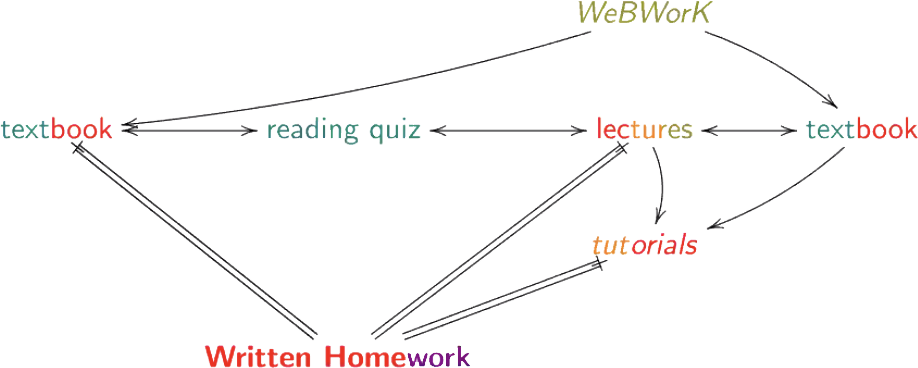
\includegraphics[width=0.75\linewidth]{Pictures/Course Structure.png}
\end{center}

Our course has multiple components. Each component is built carefully to support several aspects of the learning outcomes of our course as listed in the syllabus. This page explains how different components of the course interact with one another and helps you navigate the course

\subsubsection{Reading Quizzes}

A typical week in our course starts by doing the reading assigned for that week and ends by revisiting the reading assignment for that week.  Assigned readings are mainly from our primary textbook \cite{texbook} followed by a Quercus quiz on your assigned readings for the week and that of the previous week.  You should start your reading as soon as they are posted.

You should read all the assigned readings for the week and submit your quiz on Quercus. {\color{red}The weekly quiz is due at 10 am every Monday.} The best strategy is to spread out the reading throughout the week. You are not expected to understand everything when you read the textbook before the class. Your learning will happen gradually during lectures, tutorials, and mostly when you do the suggested problems from the textbook and the written homework.  You will need to review the textbook again after lectures. Reading Quizzes quizzes makeup 5\% of your final grade.

\subsubsection{Lectures}

\textbf{What to expect from lectures?}

 During lectures, your instructor will guide you through important concepts and invite you to participate in lecture activities. Lectures complement your reading, tutorials, and homework. Lectures are not meant to replace textbook reading. There will be concepts and theorems that are only discussed in the textbook or only during your lectures, or only in homework. You are encouraged to attend all lectures. While in your lecture you are expected to actively participate in all activities prompted by your instructor. While the delivery of the course is online, your instructor may record the lectures and make it available for you to watch asynchronously. Note that watching the lectures do not replace attending them as you will miss the in-class activities. You are asked to do a lecture reflection quiz at the end of your lecture week. The reflection due date is a day after your last lecture of the week. Reflections are a tool for your instructor to emphasize important concepts in the lectures and to collect feedback from you, and an opportunity for you to reflect on your understanding of the lecture material. Reflections are part of your participation grade as per our syllabus.

\subsubsection{Tutorials}

You must be enrolled in a tutorial.  You will have weekly tutorial sessions starting on Jan 24th. During tutorials, you will work with your classmates in small groups on tutorial worksheets.  Tutorial worksheets are carefully designed to be discussed in groups. Tutorial worksheets are roughly one week behind the lectures.

Ideally, you want to read, understand, and think about all the questions before your tutorial. This involves checking all the definitions and statements of the results you need to know to tackle questions.  Set aside 15 minutes before your tutorial to go over questions. Your tutorial sessions are facilitated by your TAs. During your tutorial, your TA will ask you to sit with your tutorial group. You will work with your groupmates on selected problems from the worksheet. Each group works on a shared document that will be checked by the TA during the tutorial. Do not expect your TA to work out the questions for you or to teach the concepts.  Your TA will give you feedback on what you already put down in your shared document. That is the more you work among your group the more your TA can help you. Your TA might choose to go over some of the questions for the entire class or answer your questions within your groups. You get the most out of your tutorials if you work on the problems ahead of time and stay active and engaged throughout the tutorial. After all, you can only get an answer to those questions you ask, either from your peers or the TA.  You will get solutions to all tutorial questions at the end of the tutorial week. Tutorials are one of the most important components of the course because they facilitate your communication with your peers.  Explain concepts to your group mates and ask them to do the same for you.  At the end of each tutorial, you will submit your shared document as a group.

This submission is marked holistically, and not for correctness. You and all your group members will receive the same mark. Your active participation in your tutorial is measured by your group submission marks. Your active participation in tutorials is part of your participation grade.

\subsubsection{Homework}
You will have four types of homework. We already talked about two of them. That is reading assignments, due weekly, as part of your Reading Quiz, and Tutorial worksheets that you work on with help of your peers during your tutorial and submit with your group.  The other two are

\itblue{WeBWork.} WeBWork is an online assignment system. You have weekly WeBWork due every Wednesday 11:59 pm.  These questions are straightforward and cover what you learned in the same week and the past week. To access the homework, you should follow the link in the assignment posted under the Homework module. You will be automatically be directed to WeBWork environment. {\color{red}WARNING:} You should check your grade for WeBWork inside the WebWork environment and not in Quercus. You may occasionally see some grades regarding this homework appear on Quercus. Those numbers are not accurate and will disappear! WeBWork makes 5\% of your final grade.

\itblue{Written Homework.}  There will be five written homework sets. These homework sets are rather long and you have about two weeks to do them. You should submit these homework sets individually. You will receive instructions on how to submit your written homework.  Only selected questions from each set are graded. The lowest grade will be dropped. Written homework sets make 10\% of your final grade.

\subsection{Lecture Rules}

\begin{itemize}
    \item Come prepared (read the textbook)
    \item Be fully present
    \begin{itemize}
        \item No distraction
        \item Ready to engage
        \item Ready to participate in activities
    \end{itemize}
    \item Reflect
    \begin{itemize}
        \item What did you learn?
        \item Engage with the textbook
        \item Write down your questions
        \item Follow up on piazza
    \end{itemize}
\end{itemize}

% ----------------------------------------------------------------------------------------------------------------------------------------------------

\chapterimage{field.jpg}
\chapter{Fields, Complex Numbers and Vector Spaces}

\section{Fields and Complex Numbers}

\subsection{Fields}

\setcounter{chapter}{5}
\setcounter{definitionT}{3}
\begin{definition}[Field]\index{Field}\index{Addition}\index{Sum}\index{Multiplication}\index{Product}
    A \term{field} is a set\footnote{Note that such set must be \bred{non-empty}.} $\mathbb{F}$ with two operations, defined on ordered pairs of elements of $\mathbb{F}$, called \term{addition} and \term{multiplication}. Addition assigns to the pair $x$ and $y \in \mathbb{F}$ their \term{sum}, which is denoted by $x + y$ and multiplication assigns to the pair $x$ and $y$ their \term{product}, which is denoted by $x \cdot y$ or $xy$. These two operations must satisfy the following properties for all $x$, $y$ and $z \in \mathbb{F}$:

    \begin{enumerate}[label=(\roman*)]
        \item Commutativity of addition $x + y = y + z$.

        \item Associativity of addition: $(x + y) + z = x + (y + z)$.

        \item Existence of an additive identity: There is an element $0 \in \mathbb{F}$, called zero, such that $x + 0 = a$.

        \item Existence of additive inverses: For each $x$ there is an element $-x \in \mathbb{F}$ such that $x + (-x) = 0$.

        \item Commutativity of multiplication: $xy  = yx$.

        \item Associativity of multiplication: $(xy)z = x(yz)$.

        \item Distributivity: $(x + y)z = xz + yz$ and $x(y + z) = xy + xz$.

        \item Existence of a multiplicative identity: There is an element $1 \in \mathbb{F}$, called $1$, such that $x \cdot 1  = x$.

        \item Existence of multiplicative inverses: If $x \neq 0$, then there is an element $x^{-1} \in \mathbb{F}$ such that $x \cdot x^{-1}  = 1$.
    \end{enumerate}
\end{definition}
\setcounter{chapter}{1}

\subsection{Complex Numbers}

Goal: build a field containing $\mathbb{R}$ such that all polynomials (such as $x^2 + 1$) have their roots.

\setcounter{chapter}{5}
\setcounter{section}{1}
\setcounter{definitionT}{1}
\begin{definition}\index{Complex Numbers}
    The set of \term{complex numbers}, denoted $\mathbb{C}$, is the set of ordered pairs of real numbers$ (a, b)$ with the operations of addition and multiplication defined by

    {~~~}

    For all $(a, b)$ and $(c, d) \in \mathbb{C}$, the \term{sum} of $(a, b)$ and $(c, d)$ is the complex number defined by $(a, b) + (c, d) = (a + c, b + d)$

    {~~~}

    and the \term{product} of $(a, b)$ and $(c, d)$ is the complex number defined by $(a, b)(c, d) = (ac - bd, ad + cb)$
\end{definition}
\setcounter{section}{2}
\setcounter{chapter}{1}

The subset of $\mathbb{C}$ consisting of those elements with second coordinate zero, $\{ (a, 0) | a \in \mathbb{R} \}$, will be identified with the real numbers in the obvious way, $a \in \mathbb{R}$ is identified with $(a, 0) \in \mathbb{C}$. If we apply our rules of addition and multiplication to the subset $\mathbb{R} \subset \mathbb{C}$, we obtain
$$(a, 0) + (c, 0) = (a + c, 0)$$
and
$$(a, 0)(c, 0) = (ac - 0 \cdot 0)(a \cdot 0 + c \cdot 0) = (ac, 0)$$

\setcounter{chapter}{5}
\setcounter{section}{1}
\setcounter{dummy}{4}
\begin{proposition}
The set of complex numbers is a field with the operations of addition and scalar multiplication as defined previously.
\end{proposition}
\setcounter{section}{2}
\setcounter{chapter}{1}

\begin{proof}
    WTS $\mathbb{C}$ is a field\footnote{To show $\mathbb{F}$ is a field, we need to check commutativity, associativity, existence of additive identity and additive inverse, multiplicative identity and multiplicative inverse, and the distributivity between addition and multiplication. }.

    (i), (ii), (v), (vi), and (vii) follow immediately.

    {~~~}

    \textbf{(iii)} The additive identity is $0 = 0 + 0i$ since

    $(0 + 0i) + (a + bi) = (0 + a) + (0 + b)i = a + bi$

    {~~~}

    \textbf{(iv)} The additive inverse of $a + bi$ is $(-a) + (-b)i$.

    $(a + bi) + ((-a) + (-b)i) = (a + (-a)) + (b + (-b))i = 0 + 0i = 0$.

    {~~~}

    \textbf{(viii)} The multiplicative identity is $1 = 1 + 0 \cdot i$ since

    $(1 + 0 \cdot i)(a + bi) = (1 \cdot a - 0 \cdot b) + (1 \cdot b + 0 \cdot a)i = a + bi$.

    {~~~}

    \textbf{(ix)} Note first that if $a + bi \neq 0$, then either $a \neq 0$ or $b \neq 0$ and $a^2 + b^2 \neq 0$. Further, note that $(a + bi)(a + (-b)i) = a^2 + b^2$.

    Therefore $\displaystyle (a + bi) \frac{a - ib}{a^2 + b^2} = 1$.

    Thus, $(a + ib)^{-1} = (a - ib) / (a^2 + b^2)$.
\end{proof}

\begin{exercise}
    Compute the following.
    \begin{enumerate}
        \item $(3-5i)^{-1}$
        {\color{lightblue} \begin{align*}
            (3-5i)^{-1}
            &=\frac{(3+5i)}{3^2+5^2}
            \\
            &=\frac{3}{34}+\frac{5}{34}i
        \end{align*} }

        \item $\displaystyle \frac{4-2i}{3-5i} = (4-2i)(3-5i)^{-1}$
        {\color{lightblue} \begin{align*}
            \frac{4-2i}{3-5i}
            &= (4-2i)(3-5i)^{-1}
            \\
            &=(4-2i) \left( \frac{1}{34}(3+5i) \right)
            \\
            &=\frac{1}{34}(4-2i)(3+5i)
            \\
            &=\frac{1}{34}(12+10+20i-6i)
            \\
            &=\frac{1}{34}(22+14i)
        \end{align*} }
    \end{enumerate}
\end{exercise}

\begin{example}
    Let $\mathbb{F}_2 = \{ 0, 1 \}$.

    \begin{center}
        \begin{tabular}{c | c c}
            \toprule
            + &0 &0 \\
            \midrule
            0 &0 &1 \\
            1 &1 &0 \\
            \bottomrule
        \end{tabular}
        \hspace{0.25\linewidth}
        \begin{tabular}{c | c c}
            \toprule
            $\times$ &0 &0 \\
            \midrule
            0 &0 &0 \\
            1 &0 &1 \\
            \bottomrule
        \end{tabular}
    \end{center}

    \textbf{Discussion}

    \begin{itemize}
        \item Is $+$ commutative? How to see it visually?

        \begin{itemize}
            \item Yes.

            \item The diagonals align up (this tabel is symmetric).
        \end{itemize}

        \item Is $\times$ commutatiove? How to see it visually?

        \begin{itemize}
            \item Yes.

            \item The diagonals align up (this tabel is symmetric).
        \end{itemize}

        \item Does $(\mathbb{F}_2, +, \times)$ have additive and multiplicative identities? How to see them visually?

        \begin{itemize}
            \item Yes, they all have their identities.

            \item $0$ is the additive identity.

            The corresponding rows and columns of $0$ are copies of the index row/column.

            \item $1$ is the multiplicative identity.

            The corresponding rows and columns of $1$ are copies of the index row/column.
        \end{itemize}
    \end{itemize}
\end{example}

\section{Vector Spaces}

\subsection{Vector Space}

Let $\mathbb{F}$ be a field\footnote{The differences between a field and a vector space: \begin{itemize} \item Over \term{fields}, we have two binary operations; \item Over \term{vector spaces}, we have one binary operation and one scalar multiplication. \end{itemize}}.

\setcounter{chapter}{5}
\setcounter{section}{2}
\begin{definition}[Vector Space over a Field]\index{Vector Space over a Field}
    A \term{vector space over $\mathbb{F}$} is a set $V$ (whose elements are called \term{vectors}) together with two operations:
    \begin{itemize}
        \item A binary operation called \bred{vector addition}, which for each pair of vectors $\vec{v}, \vec{w} \in V$ produces a vector denoted $\vec{v} + \vec{w} \in V$, and

        \item an operation called \bred{multiplication by a scalar}\footnote{This is also called a \bred{scalar multiplication}} (a field element), which for each vector $\vec{v} \in V$, and each scalar $c \in \mathbb{F}$ produces a vector denoted $c\vec{v}\in V$.
    \end{itemize}
\end{definition}
\setcounter{section}{3}
\setcounter{chapter}{1}

\begin{minipage}[t]{0.45\linewidth}
    $$\begin{matrix} &+: &V\times V  &\to &V \\& &(\vec{v},\vec{w}) &\mapsto &\vec{v}+\vec{w} \end{matrix}$$
\end{minipage}
\begin{minipage}[t]{0.45\linewidth}
    $$\begin{matrix} &\times: &\mathbb{F}\times V  &\to &V \\& &(c,\vec{v}) &\mapsto &c\vec{v} \end{matrix}$$
\end{minipage}

Furthermore, the two operations must satisfy the following axioms:

\begin{enumerate}[label=(\arabic*)]
    \item For all vectors $\vec{u}$, $\vec{v}$, and $\vec{w} \in V$, $(\vec{u} + \vec{v}) + \vec{w} = \vec{u} + (\vec{v} + \vec{w})$. (addition is \term{associative})

    \item For all vectors $\vec{v}$ and $\vec{w} \in V$, $\vec{v} + \vec{w} = \vec{w} + \vec{v}$. (addition is \term{commutative})

    \item There exists a vector $\vec{0} \in V$ with the property that $\vec{v} + \vec{0} = \vec{v}$ for all vectors $\vec{v} \in V$. ($\exists$ an \term{additive identity})

    \item For each vector $\vec{v} \in V$, there exists a vector denoted $-\vec{v}$ with the property that $\vec{v} + -\vec{v} = \vec{0}$. ($\exists$ \term{additive inverse})

    \item For all vectors $\vec{v}$ and $\vec{w} \in V$  and all scalars $c \in \mathbb{F}$, $c(\vec{v}+ \vec{w}) = c\vec{v} + c\vec{w}$. (\term{distributive} property 1)

    \item For all vectors $\vec{v} \in V$, and all scalars $c$ and $d \in \mathbb{F}$, $(c + d)\vec{v} = c\vec{v} + d\vec{v}$. (\term{distributive} property 2)

    \item For all vectors $\vec{v} \in V$, and all scalars $c$ and $d \in \mathbb{F}$, $(cd)\vec{v} = c(d\vec{v})$. (multiplication is \term{associative})

    \item For all vectors $\vec{v} \in V$, $1\vec{v} = \vec{v}$. ($\exists$ an \term{multiplicative identity})
\end{enumerate}

\begin{example}
{~~~}

    Define $\mathbb{R}^n = \left\{ \begin{pmatrix} a_1\\\vdots\\a_n \end{pmatrix}, a_i \in \mathbb{R} \right\}$, 
    $\mathbb{C}^n = \left\{ \begin{pmatrix} z_1\\\vdots\\z_n \end{pmatrix}, a_i \in \mathbb{C} \right\}$. 
    
    Take $\vec{z} = \begin{pmatrix} z_1 \\ \vdots \\ z_n \end{pmatrix}$, $\vec{w} = \begin{pmatrix} w_1 \\ \vdots \\ w_n \end{pmatrix}$, then $\vec{z} + \vec{w} = \begin{pmatrix} z_1 + w_1 \\ \vdots \\ z_n + w_n \end{pmatrix}$\footnote{Note that the two $+$'s ($\vec{z} + \vec{w}$ and $z_i + w_i$) here are different. The former is vector addition, while the later is addition over $\mathbb{C}$. }.
    
    In general, $\mathbb{F}^n := \left\{ \begin{pmatrix} a_1 \\ \vdots \\ a_n \end{pmatrix}, a_i \in \mathbb{F} \right\}$ is a vector space over the field $\mathbb{F}$~\footnote{``A vector space over the field $\mathbb{F}$'' can be shortened to ``$\mathbb{F}$ vector space'', or ``$\mathbb{F}$\_V.S.''. }. 
    
    \begin{itemize}
        \item Additive identity: $\vec{0} := \begin{pmatrix} 0 \\ \vdots \\ 0 \end{pmatrix}$\footnote{Note that $\vec{0}$ is the additive identity of $\mathbb{F}^n$, while the $0$’s are the additive identity over the field $\mathbb{F}$.}

        \item Take $\vec{v} = \begin{pmatrix} v_1 \\ \vdots \\ v_n \end{pmatrix} \in \mathbb{F}^n$, then $-\vec{v} = \begin{pmatrix} -v_1 \\ \vdots \\ -v_n \end{pmatrix}$~\footnote{Note that the two $-$'s ($-\vec{v}$ and $-v_i$) here are different. The former is the symbol for the additive inverse inside $\mathbb{F}^n$, while the later is additive inverse over the field $\mathbb{F}$. }. 
    \end{itemize}
\end{example}

\begin{example}
{~~~}

    Define $\mathcal{P}_n(\mathbb{F}) = \left\{ a_0 + a_1x + a_2x^2 + \cdots + a_nx^n ~|~a_i \in \mathbb{F} \right\}$. 
    
    \begin{itemize}
        \item $\mathcal{P}_n(\mathbb{F})$ is an $\mathbb{F}$\_V.S. 
        
        Take $p(x) = a_0 + a_1x + \cdots + a_nx^n$, $q(x)=b_0 + b_1x + \cdots + b_nx^n \in P_n(\mathbb{F})$. 
        
        $p(x)+q(x):=(a_0+b_0)+(a_1+b_1)x+\dots+(a_nb_n)x^n$. 
        
        $cp(x) := ca_0 + \overbrace{ca_1}^{c ~\times~ a_1 \mathrm{~on~}\mathbb{F}}x + \cdots + ca_nx^n$. 
    \end{itemize}
\end{example}

\begin{example}
{~~~}

    $F(\mathbb{R}) := \left\{ f:\mathbb{R} \to \mathbb{R} ~|~f \text{ is a function} \right\}$ is a real vector space. 
    
    Consider $f(x) = x^2 \in F(\mathbb{R})$. 
    $$\begin{matrix} &f: &\mathbb{R} &\to &\mathbb{R} \\& &x &\mapsto &x^2 \end{matrix}$$
    \begin{center}
        \begin{tikzpicture}
            \draw[->] (-2.5, 0) -- (2.5, 0) node[right] {$x$};
            \draw[->] (0, -1) -- (0, 4) node[above] {$y$};
            \draw[scale=1.0, domain=-2:2, smooth, variable=\x, red] plot ({\x}, {\x*\x});
        \end{tikzpicture}
    \end{center}
    
    \begin{itemize}
        \item Define vector addition and scalar multiplication
        
        Take $f,g \in F(\mathbb{R})$. 
        \begin{itemize}
            \item $(f+g)(x):=f(x)+g(x)$ for all $x \in \mathbb{R}$.

            \item $(rf)(x)=r\left(f(x)\right)$ for all $x \in \mathbb{R}$ and all $x \in \mathbb{R}$. 
        \end{itemize}
        
        \item Additive identity of $F(\mathbb{R})$:
        $$\begin{matrix} &\underset{F(\mathbb{R})}{0} &\mathbb{R} &\to &\mathbb{R} \\& &x &\mapsto &0_{\mathbb{R}} \end{matrix}$$
        
        \begin{itemize}
            \item Prove that $\underset{F(\mathbb{R})}{0}$ is the additive identity of $F(\mathbb{R})$.
            
            \begin{proof}
                WTS $\forall f \in F(\mathbb{R})$, $f+\underset{F(\mathbb{R})}{0} = f$. 
                
                Pick arbitrary $f \in F(\mathbb{R})$, $f: \mathbb{R} \to \mathbb{R}$. 
                
                WTS $\forall x \in \mathbb{R}$, $(f+\underset{F(\mathbb{R})}{0})(x) = f(x)$. 
                
                \begin{flalign*}
                    \text{Pick }x \in \mathbb{R}, 
                    (f+\underset{F(\mathbb{R})}{0})(x)
                    &=f(x)+\underset{F(\mathbb{R})}{0}(x)
                    &\text{by the definition of}+\text{in }F(\mathbb{R})
                    &&\\
                    &=f(x)+0_{\mathbb{R}}
                    &\text{by the definition of}\underset{F(\mathbb{R})}{0}
                    \\
                    &=f(x)
                    &\text{since }0_{\mathbb{R}}\text{ is the additive identity in }\mathbb{R}
                \end{flalign*}
                
                We have shown that $\forall x \in \mathbb{R}$, $(f+\underset{F(\mathbb{R})}{0})(x) = f(x)$. 
            \end{proof}
            
            \item Prove that $\forall f \in F(\mathbb{R})$, $\exists -f \in F(\mathbb{R})$ s.t. $f + (-f) = \underset{F(\mathbb{R})}{0}$. 
            \begin{proof}
                WTS $\forall f \in F(\mathbb{R})$, $\exists -f \in F(\mathbb{R})$ s.t. $f + (-f) = \underset{F(\mathbb{R})}{0}$. 
                
                Pick arbitrary $f \in F(\mathbb{R})$. 
                
                Let $-f$ be the function $$\begin{matrix} -f: &\mathbb{R} &\to &\mathbb{R} \\ &x &\mapsto &-f(x) \end{matrix}$$
                
                WTS $f+(-f)=\underset{F(\mathbb{R})}{0}$. 
                
                WTS $\forall x \in \mathbb{R}$, $(f+(-f))(x) = \underset{F(\mathbb{R})}{0}(x)$.  
                
                {~~~}
                
                Pick arbitrary $x \in \mathbb{R}$.  
                \begin{flalign*}
                    (f+(-f))(x)
                    &=f(x)+(-f)(x)
                    &\text{by the definition of}+\text{in }\mathbb{R}
                    \\
                    &=f(x)+(-f(x))
                    &\text{by the definition of}-f
                    \\
                    &=\underset{\mathbb{R}}{0}
                    &\text{since }\underset{\mathbb{R}}{0}\text{ is the additive identity in }\mathbb{R}
                    \\
                    &=\underset{F(\mathbb{R})}{0}
                    &\text{since}\forall x \in \mathbb{R},\underset{F(\mathbb{R})}{0}(x)=\underset{\mathbb{R}}{0}
            \end{flalign*}
            
            Thus, $\forall f \in F(\mathbb{R})$, $\exists -f \in F(\mathbb{R})$ s.t. $f + (-f) = \underset{F(\mathbb{R})}{0}$. 
            \end{proof}
        \end{itemize}
    \end{itemize}
\end{example}

\begin{example}
    Prove $\underset{2 \times 3}{M}(\mathbb{R}) \left\{ [a_{ij}] ~|~ a_{ij} \in \mathbb{R} \right\}$ is a vector space. 
    
    Example: $\begin{bmatrix}  1 &2 &0 \\ 0 &0 & 0 \end{bmatrix} \in \underset{2 \times 3}{M}(\mathbb{R})$. 
    \begin{itemize}
        \item $\begin{bmatrix} a_{ij} \end{bmatrix} + \begin{bmatrix} b_{ij} \end{bmatrix} = \begin{bmatrix} a_{ij}+b_{ij} \end{bmatrix}$

        \item $r\begin{bmatrix} a_{ij} \end{bmatrix} = \begin{bmatrix} ra_{ij} \end{bmatrix}$

        \item Additive identity in $\underset{2\times3}M(\mathbb{R})$ is $\underset{2\times3}{0} = \begin{bmatrix} 0&0&0\\0&0&0 \end{bmatrix}$. 

        \item Given $A = \begin{bmatrix} a_{ij} \end{bmatrix} \in \underset{2\times3}M(\mathbb{R})$, $-A = \begin{bmatrix} -a_{ij} \end{bmatrix}$ is the additive inverse of $A$. 
    \end{itemize}
\end{example}

\setcounter{section}{1}
\setcounter{dummy}{5}
\begin{proposition}
    Let $V$ be a vector space. Then 
    
    \begin{enumerate}[label=\alph*)]
        \item The zero vector $\vec{0}$ (additive identity in $V$) is unique.
        \begin{proof}
            WTS Additive identity in $V$ is unique\footnote{To prove that something is unique, a common technique is to assume we have two examples of the object in question, then show that those two examples must in fact be equal. }.

            Suppose $\vec{0}$ and $\vec{0}'$ are additive identity in $V$. 
            
            Since $\vec{0}$ is additive identity, $\forall \vec{v} \in V$, $\vec{v} + \vec{0} = \vec{v}$. In particular, $\vec{0}' + \vec{0} = \vec{0}'$. 
            
            Since $\vec{0}'$ is additive identity, $\forall \vec{v} \in V$, $\vec{v} + \vec{0}' = \vec{v}$. In particular, $\vec{0} + \vec{0}' = \vec{0}$. 

            So $\vec{0}' = \vec{0} + \vec{0}' = \vec{0}$, so there is only one additive identity in $V$.
        \end{proof}

        \item For all $\vec{v} \in V$ , $\underset{\mathbb{F}}{0}\vec{v} = \vec{0}_V$.

        \begin{proof}
            WTS $\forall \vec{v} \in V$, $\underset{\mathbb{F}}{0}\vec{v} = \vec{0}_V$. 
            
            Pick $\vec{v} \in V$. 
            \begin{align*}
                \underset{\mathbb{F}}{0}\vec{v} 
                &= (\underset{\mathbb{F}}{0} + \underset{\mathbb{F}}{0})\vec{v} 
                \\
                &= \underset{\mathbb{F}}{0}\vec{v} + \underset{\mathbb{F}}{0}\vec{v}
                \\
                (-\underset{\mathbb{F}}{0}\vec{v}) + \underset{\mathbb{F}}{0}\vec{v}
                &= (-\underset{\mathbb{F}}{0}\vec{v}) + (\underset{\mathbb{F}}{0}\vec{v} + \underset{\mathbb{F}}{0}\vec{v})
                \\
                -\underset{\mathbb{F}}{0}\vec{v} + \underset{\mathbb{F}}{0}\vec{v}
                &= (-\underset{\mathbb{F}}{0}\vec{v} + \underset{\mathbb{F}}{0}\vec{v}) + \underset{\mathbb{F}}{0}\vec{v}
                \\
                \vec{0}_V
                &=
                \vec{0}_V + \underset{\mathbb{F}}{0}\vec{v}
                \\
                &=\underset{\mathbb{F}}{0}\vec{v}
            \end{align*}
            
            Thus, $\forall \vec{v} \in V$, $\underset{\mathbb{F}}{0}\vec{v} = \vec{0}_V$. 
        \end{proof}

        \item For each $\vec{v} \in V$, the additive inverse $-\vec{v}$ is unique.

        \begin{proof}
            We use the same idea as in the proof of part a. Given $\vec{v} \in V$, if $-\vec{v}$ and $(-\vec{v})'$ are two additive inverses of $\vec{v}$, then on one hand we have $\vec{v} + -\vec{v}  + (-\vec{v})' = (\vec{v} + -\vec{v}) + (-\vec{v})' = \vec{0} + (-\vec{v})' = (-\vec{v})'$, by axioms 1, 4, and 3. On the other hand, if we use axiom 2 first before associating, we have $\vec{v} + -\vec{v}  + (-\vec{v})' = \vec{v} + (-\vec{v})' + -\vec{v} = (\vec{v} + (-\vec{v})') + -\vec{v} = \vec{0} + -\vec{v} = -\vec{v}$. Hence $-\vec{v} = (-\vec{v})'$, and the additive inverse of $\vec{v}$ is unique.
        \end{proof}
        
        \item For all $\vec{v} \in V$, and all $c \in \mathbb{R}$, $(-c)\vec{v}  = -(c\vec{v})$.
        \begin{proof}
            We have $c\vec{v} + (-c)\vec{v} = (c + -c)\vec{v} = 0\vec{v} = \vec{0}$ by axiom 6 and part b. Hence $(-c)\vec{v}$ also serves as an additive inverse for the vector $c\vec{v}$. By part c, therefore, we must have $(-c)\vec{v} = -(c\vec{v})$.
        \end{proof}
    \end{enumerate}
\end{proposition}
\setcounter{section}{3}

\subsection{Subspace}
\begin{example}
    Let $W \subseteq \mathbb{R}^3$. 
    
    Let $\vec{w}_1, \vec{w}_2 \in W$. 
    
    Then, $\vec{w}_1 + \vec{w}_2 \in W$. 
    $$
        \begin{matrix} +: &W\times W &\to &W \\ &(\vec{w}_1, \vec{w}_2) &\mapsto &\vec{w}_1 + \vec{w}_2 \end{matrix} 
        \qquad \qquad 
        \begin{matrix} \cdot: &\mathbb{R} \times W &\to &W \\ &(r, \vec{w}) &\mapsto &r\vec{w} \end{matrix}
    $$
    
    We can conclude that $W$ is a subspace of $\mathbb{R}^3$~\footnote{A short hand of ``$W$ \textit{is a subspace of} $V$'' is ``$W \underset{S.S.}{\subseteq} V$''. }. 
\end{example}

\setcounter{section}{2}
\setcounter{definitionT}{5}
\begin{definition}[Subspace]\index{Subspace}
    Let $V$ be a vector space and let $W \subseteq V$ be a \itblue{non-empty} subset. Then $W$ is a (vector) \term{subspace} of $V$ if $W$ is a vector space itself under the operations of vector sum and scalar multiplication from $V$.
\end{definition}
\setcounter{section}{3}

\setcounter{section}{2}
\setcounter{dummy}{7}
\begin{theorem}[Subset Test]
    Let $V$ be a vector space, and let $W$ be a non-empty subset of $V$. Then $W$ is a subspace of $V$ if and only if for all $\vec{v}, \vec{w} \in W$, and all $c \in \mathbb{R}$. we have $c\vec{v} + \vec{w} \in W$~\footnote{This is equivalent to ``$W$ is closed under vector addition and under scalar multiplication of $V$''. }.
\end{theorem}
\setcounter{section}{3}

\begin{example}
    Is $\mathbb{R}^2$ a subspace of $\mathbb{R}^3$? 
    
    Note that $\mathbb{R}^2 = \left\{ \begin{bmatrix}a _1 \\ a_2 \end{bmatrix} ~|~ a_1,a_2 \in \mathbb{R} \right\}$ but $\mathbb{R}^3 = \left\{ \begin{bmatrix}a _1 \\ a_2 \\ a_3 \end{bmatrix} ~|~ a_1,a_2,a_3 \in \mathbb{R} \right\}$. Clearly, $\mathbb{R}^2 \not\subseteq \mathbb{R}^3$. 
\end{example}

\begin{example}
    Let $\mathbb{F}$ be a field. 
    
    Define $\mathbb{F}^3 = \left\{ \begin{bmatrix} a_1\\a_2\\a_3 \end{bmatrix} ~|~ a_i \in \mathbb{F} \right\}$. 
    
    Let $W = \left\{ \begin{bmatrix}a_1\\a_2\\a_3\end{bmatrix} \in \mathbb{F}^3 ~|~ a_1+a_2+a_3=\underset{\mathbb{F}}{0} \right\}$. 
    
    \begin{proof}
        WTS $W$ is a subspace of $\mathbb{F}^3$. 
        
        \begin{itemize}
            \item Show that $W$ is non-empty. 

            $\begin{bmatrix} 0\\0\\0 \end{bmatrix} \in W$, so $W$ is non-empty. 

            \item Show that $W \subseteq \mathbb{F}^3$. 
            
            Since $\forall \vec{v} \in W$, $\vec{v} \in \mathbb{F}^3$, we have $W \subseteq \mathbb{F}^3$. 
            
            \item Show that $W$ is closed under vector addition. 

            Let $\vec{w}_1 = \begin{bmatrix}a_1\\a_2\\a_3\end{bmatrix}, \vec{w}_2 = \begin{bmatrix}b_1\\b_2\\b_3\end{bmatrix} \in W$, $a_i,b_i \in \mathbb{F}$. 
            
            Then, $\vec{w}_1 + \vec{w}_2 = \begin{bmatrix}a_1+b_1\\a_2+b_2\\a_3+b_3\end{bmatrix}$. 
            
            Note that $(a_1+b_1) + (a_2+b_2) + (a_3+b_3) = (a_1+a_2+a_3) + (b_1+b_2+b_3) = \underset{\mathbb{F}}{0}+\underset{\mathbb{F}}{0}=\underset{\mathbb{F}}{0}$. 
            
            Thus, $\vec{w}_1 + \vec{w}_2 \in W$. 
            
            That is, $W$ is closed under vector addition.

            \item Show that $W$ is closed under scalar multiplication. 
            
            Pick $r \in \mathbb{F}$, pick $\vec{w} \in W$. 
            
            $r\vec{w} = r\begin{bmatrix}a_1\\a_2\\a_3\end{bmatrix} = \begin{bmatrix}ra_1\\ra_2\\ra_3\end{bmatrix}$. 
            
            $ra_1+ra_2+ra_3 = r(a_1+a_2+a_3) = r(\underset{\mathbb{F}}{0}) = \underset{\mathbb{F}}{0}$. 
            
            Thus, $r\vec{w} \in W$. 
            
            Thus is, $W$ is closed under scalar multiplication. 
        \end{itemize}
        
        Thus, $W \underset{S.S.}{\subseteq} \mathbb{F}^3$. 
    \end{proof}
\end{example}

\section{Linear Combinations}

\setcounter{section}{3}
\setcounter{definitionT}{0}
\begin{definition}\index{Linear Combination}\index{Empty Set of a Vector Space}\index{Span}
    Let $S$ be a subset of a vector space $V$.
    
    \begin{itemize}
        \item A \term{linear combination} of vectors in $S$ is any sum $a_x\vec{v}_1 + \cdots + a_n\vec{v}_n$, where the $a_i \in \mathbb{R}$, and the $\vec{v}_i \in S$.

        \item If $5 \neq \emptyset$ (the empty subset of $V$), the set of all linear combinations of vectors in $S$ is called the (linear) \term{span} of $S$, and denoted $\mathrm{Span}(S)$. If $S = \emptyset$, we define $\mathrm{Span}(S) = \{ \vec{0} \}$.

        \item If $W = \mathrm{Span}(S)$, we say $S$ \term{spans} (or generates) $W$.

        \item We think of the span of a set $S$ as the set of all vectors that can be ``built up'' from the vectors in S by forming linear combinations.
    \end{itemize}
\end{definition}
\setcounter{section}{4}

{~~~}

How do we describe $\mathrm{Span}(S)$ in set builder notation? 
\begin{itemize}
  \item If $S$ is finite or infinite 
  $$\mathrm{Span}(S) = \{ a_1\vec{x}_1 + a_2\vec{x}_2 + \cdots + a_n\vec{x}_n ~|~ a_i \in \mathbb{F}, n \in \mathbb{N}, \vec{x}_i \in S \}$$

  \item If $S$ is finite 
  $$S = \{ \vec{w}_1 , \dots, \vec{w}_n \}$$ 
  $$\mathrm{Span}\left( S \right) = \{ a_1\vec{w}_1 + \cdots + a_k\vec{w}_k ~|~ a_i \in \mathbb{F}, \vec{w}_i \in S \}$$
\end{itemize}

\begin{example}
{~~~}

\begin{minipage}[t]{0.45\linewidth}
    Let $S = \{ \sin^2x,\cos^2x \} \subseteq F(\mathbb{R})$. 
    
    \begin{itemize}
        \item Describe $\mathrm{Span}(S)$. 

        {\color{lightblue} $\mathrm{Span}\left( S \right) = \{ a_1\sin^2x+a_2\cos^2x ~|~ a_i \in \mathbb{R} \}$ }
        
        \item True or False: $\mathrm{Span}(S)$ contains all constant functions 

        {\color{lightblue} True. 
        
        Let $f(x)=c$, $c \in \mathbb{R}$. 
        \begin{flalign*}
            \text{Then, }
            f(x) 
            &= c \cdot 1
            &&\\
            &=c(\sin^2x+\cos^2x)
            \\
            &=c\sin^2x+c\cos^2x
            \in \mathrm{Span}\left( S \right)
            \end{flalign*} }
    \end{itemize}
\end{minipage}
\begin{minipage}[t]{0.45\linewidth}
    Let $S' = \left\{ \begin{bmatrix} 1&0\\0&0 \end{bmatrix}, \begin{bmatrix} 0&1\\0&0 \end{bmatrix} \right\} \subseteq \underset{2\times2}{M}(\mathbb{R})$.     
    
    \begin{itemize}
        \item Describe $\mathrm{Span}(S)$. 

        {\color{lightblue} $\mathrm{Span}\left( S \right) = \left\{ \begin{bmatrix} a_1&a_2\\0&0 \end{bmatrix} ~|~ a_1,a_2 \in \mathbb{R} \right\}$ }
        
        \item True or False: $\mathrm{Span}\left( S' \right)$ contains no symmetric matrix. 

        {\color{lightblue} False.
        
        Consider $0_{2\times2}=\begin{bmatrix} 0&0\\0&0 \end{bmatrix}$. }
    \end{itemize}
\end{minipage}
\end{example}

\begin{example}
    Let $\mathcal{P}(\mathbb{R}):=$ the set of all polynomials with real coefficients. 

    \begin{itemize}
        \item Give s spanning set for $\mathcal{P}(\mathbb{R})$. 
        $$\color{lightblue} S = \{ x^i ~|~ i \in \mathbb{N} \cup \{0\} \} $$
        
        \vspace{-0.5cm}
        \item Can we find a finite spanning set for ? 

        {\color{lightblue} No. }
    \end{itemize}
\end{example}

\setcounter{dummy}{3}
\begin{theorem}
    Let $V$ be a vector space and let $S$ be any subset of $V$. Then $\mathrm{Span}(S)$ is a subspace of $V$.
\end{theorem}

% TODO: complete the proof
\begin{proof}
    $V$ is an $\mathbb{F}$\_V.S. $S \subseteq V$. WTS $\mathrm{Span}(S) \underset{S.S.}{\subseteq} V$. 
    
    \begin{itemize}
        \item Show $\mathrm{Span}(S) \subseteq V$. 
        
        Pick $\vec{v} \in \mathrm{Span}\left( S \right) = \{ a_1\vec{v}_1 + \cdots + a_m\vec{v}_m ~|~ a_i \in \mathbb{F}, \vec{v}_i \in S, m \in \mathbb{N} \}$. 
        
        Then, $\vec{v} = a_1\vec{v}_1 + \cdots + a_m\vec{v}_m$ for some $\vec{v}_1, \dots, \vec{v}_m \in S$ and $a_1,\dots a_m  \in \mathbb{F}$. 
        
        Since $\vec{v}_i \in S \subseteq V$, $\vec{v}$ is a linear combination of vectors in $V$, and $V$ is a vector space. 
        
        Thus, $\vec{v} \in V$. 
        
        \item Show $\mathrm{Span}(S) \neq \emptyset$

        \item Show $\mathrm{Span}(S)$ is closed under vector addition. 

        \item Show $\mathrm{Span}(S)$ is closed under scalar multiplication. 
    \end{itemize}
\end{proof}

\begin{example}
{~~~}
    
    Let $S_1=\{ 1, 2\sin^2{x}, 3\cos^2{x} \}$, $S_2 = \{ \sin^2{x}, \cos^2{x} \}$. 
    
    $\mathrm{Span}(S_1) \overset{?}= \mathrm{Span}(S_2)$? 
    
    \begin{itemize}
        \item $\mathrm{Span}\left( S_1 \right) \overset{?}{\subseteq} \mathrm{Span}\left( S_2 \right)$? 
        
        {\color{lightblue} Yes. 
        
        $S_1 \subseteq \mathrm{Span}\left( S_2 \right)$. 
        
        $\vec{v} = a\underset{\in \mathrm{Span}\left( S_2 \right)}{\sin^2x}+b\underset{\in\mathrm{Span}\left( S_2 \right)}{\cos^2x} \in \mathrm{Span}\left( S_2 \right)$ since $\mathrm{Span}\left( S_2 \right) \underset{S.S.}{\subseteq} V$. }
        
        \item $\mathrm{Span}\left( S_2 \right) \overset{?}{\subseteq} \mathrm{Span}\left( S_1 \right)$? 
        
        {\color{lightblue} Yes. 
        
        $S_2 \subseteq \mathrm{Span}\left( S_1 \right)$. 
        
        $\vec{v} = a \cdot \underset{\in\mathrm{Span}\left( S_1 \right)}{1} + b \underset{\in \mathrm{Span}\left( S_1 \right)}{\sin^2x} + c \underset{\in\mathrm{Span}\left( S_1 \right)}{\cos^2x} \in \mathrm{Span}\left( S_1 \right)$ since $\mathrm{Span}\left( S_1 \right) \underset{S.S.}{\subseteq} V$. }

    \end{itemize}
\end{example}

\section{Linear Dependence and Linear Independence}

\setcounter{section}{4}
\setcounter{definitionT}{1}
\begin{definition}[Linear Dependence]\index{Linear Dependence}
    Let $V$ be a vector space, and let $S$ be a subset of $V$.
    
    \begin{enumerate}[label=\alph*)]
        \item A \term{linear dependence}\footnote{A linear dependence is often called a \bred{non}\itblue{-trivial relation}. } among the vectors of S is an equation $$a_1\vec{v}_1 + \cdots + a_n\vec{v}_n = 0$$ where the $\vec{v}_i \in S$ and the $a_i \in \mathbb{R}$ are not all zero (i.e., at least one of the $a_i \neq 0$).

        \item the set $S$ is said to be \term{linearly dependent} if there exists a linear dependence among the vectors in $S$.
    \end{enumerate} 
\end{definition}
\setcounter{section}{5}

\begin{example}
{~~~}

    Is $S = \left\{ \begin{bmatrix} 1&2\\3&4 \end{bmatrix}, \begin{bmatrix} 0&1\\2&3 \end{bmatrix}, \begin{bmatrix} 0&0\\0&0 \end{bmatrix} \right\} \subseteq \underset{2\times2}{M}(\mathbb{R})$ linearly independent? 
    
    {\color{lightblue} Yes. $$0 \begin{bmatrix} 1&2\\3&4 \end{bmatrix} + 0 \begin{bmatrix} 0&1\\2&3 \end{bmatrix} + 1 \begin{bmatrix} 0&0\\0&0 \end{bmatrix} = \vec{0}_{2\times2}$$ }
\end{example}

\begin{example}
    Let $V$ be a vector space over the field $\mathbb{F}$. 
    
    Is $S' = \{\vec{0}, \vec{v}_1, \dots, \vec{v}_n\} \subseteq V$ linearly independent? 
    
    {\color{lightblue} Yes. $$1_{\mathbb{F}}\vec{0} + 0_{\mathbb{F}}\vec{v}_1 + \cdots + 0_{\mathbb{F}}\vec{v}_n = \vec{0}$$ }
\end{example}

\setcounter{section}{4}
\setcounter{definitionT}{3}
\begin{definition}[Linearly Independent]\index{Linear Independence}
    A subset $S$ of a vector space $V$ is \term{linearly independent} if whenever we have $a_i \in \mathbb{R}$ and $\vec{v}_i \in S$ such that $a_1\vec{v}_1 + \cdots + a_n\vec{v}_n = 0$, then $a_i = 0$ for all $i$.
\end{definition}
\setcounter{section}{5}

\begin{example}
    Is $S = \{ e^x, e^{2x}, e^{3x} \} \subseteq \mathcal{C}(\mathbb{R})$ linearly independent? 
    
    {\color{lightblue} No. 
    
    {~~~}
    
    Assume $\forall x \in \mathbb{R}, a_1e^x + a_2e^{2x} + a_3e^{3x} = \vec{0}$. 
    
    In particular when $x = 0$, $a_1+a_2+a_3 = 0$. 
    
    {~~~}

    Taking the derivative on both sides. $\forall x \in \mathbb{R}$, $a_1e^x+2a_2e^{2x}+3a_3e^{3x}=\vec{0}$. 
    
    Again, when $x = 0$, $a_1+2a_2+3a_3 = 0$. 
    
    {~~~}

    Take the derivative again, $\forall x \in \mathbb{R}$, $a_1e^x+4a_2e^{2x}+9a_3e^{3x}=\vec{0}$.
    
    When $x = 0$, $a_1+4a_2+9a_3 = 0$.
    
    {~~~}

    Thus, $a_1 = a_2 = a_3 = 0$. 

    So $S$ is linearly independent. }
\end{example}

\setcounter{section}{4}
\setcounter{dummy}{6}
\begin{proposition}
{~~~}

    \begin{itemize}
        \item Let $S$ be a linearly dependent subset of a vector space $V$, and let $S'$ be another subset of $V$ that \bred{contains} $S$. Then $S'$ is also linearly dependent.

        \item Let $S$ be a linearly independent subset of a vector space $V$ and let $S'$ be another subset of $V$ that is \bred{contained in} $S$. Then $S'$ is also linearly independent.
    \end{itemize}
\end{proposition}
\setcounter{section}{5}

\begin{example}
    Let $S_1$ and $S_2$ be linearly independent subsets of a vector space $V$. 
    
    \begin{enumerate}[label=\alph*)]
        \item Is $S_1 \cup S_2$ always linearly independent? Why or why not? 
            
            {\color{lightblue} No.
            
            $\{ 1 \} \in \mathbb{R}$, $\{ 2 \} \in \mathbb{R}$ and they are linearly independent. 
            
            $\{ 1 \} \cup \{2 \} = \{1, 2\} \in \mathbb{R}$ and it is linearly dependent. }

        \item Is  always linearly independent? Why or why not? 

            {\color{lightblue} Yes. 
            
            $S_1 \cap S_2 \subseteq S_1$ and $S_1 \cap S_2 \subseteq S_2$. Then by the proposition $S_1 \cap S_2$ is linearly independent. }

        \item Is  always linearly independent? Why or why not? 

            {\color{lightblue} Yes. 
            
            $S_1 \setminus S_2 \subseteq S_1$. Then by the proposition $S_1 \setminus S_2$ is linearly independent. }

    \end{enumerate}
\end{example}

\setcounter{section}{6}
\setcounter{dummy}{7}
\begin{lemma}
    Let $S$ be a linearly independent subset of $V$ and let $\vec{v} \in V$, but $\vec{v} \notin S$. Then $S \cup \{\vec{v}\}$ is linearly independent if and only if $\vec{v} \notin \mathrm{Span}\left( S \right)$. 
\end{lemma}
\setcounter{section}{5}

\begin{proof}
    WTS $S \cup \{\vec{v}\}$ is linearly independent if and only if $\vec{v} \notin \mathrm{Span}((S)$. 
    
    \begin{itemize}
        \item $\rightarrow$: Assume $S \cup \{ \vec{v} \}$ is linearly independent. WTS $\vec{v} \notin \mathrm{Span}\left( S \right)$. 
        
        {~~~}
        
        Proof by contradiction. Assume $\vec{v} \in \mathrm{Span}(S)$. 

        Then, $\exists r_1, \dots, r_m \in \mathbb{F}$, $\vec{s}_1, \dots, \vec{s}_m \in S$ s.t. $\vec{v} + r_1\vec{s}_1 + \cdots + r_m\vec{s}_m$.
        
        i.e $\vec{v} - r_1\vec{s}_1 - \dots - r_m\vec{s}_m = \vec{0}$. This is a non-trivial relation among vectors in $S \cup \{ \vec{v} \}$, $S \cup \{ \vec{v} \}$ is linearly dependent. 

        Contradiction with the assumption. 
        
        {~~~}
        
        Thus, $\vec{v} \notin \mathrm{Span}\left( S \right)$. 
 
        \item $\leftarrow$: Assume $\vec{v} \notin \mathrm{Span}(S)$. WTS $S \cup \{ \vec{v} \}$ is linearly independent. 
        
        {~~~}
        
        (Prove the contrapositive $\lnot ( S \cup \{ \vec{v}\} \text{ is linearly independent} ) \implies \lnot \left( \vec{v} \notin \mathrm{Span}(S) \right)$, that is, we prove that ``$S \cup \{ \vec{v}\} \text{ is linearly dependent} \implies \vec{v} \in \mathrm{Span}(S)$''). 
        
        {~~~}
        
        There exists a dependency relation among vectors in $S \cup \{\vec{v} \}$. 
        
        This relation should contain $\vec{v}$. 
        
        $\exists r_1, \dots, r_m, a \in \mathbb{F}$ s.t. $r_1\vec{s}_1 + \cdots + r_m\vec{s}_m+a\vec{v} = \vec{0}$. 
        \begin{flalign*}
            \text{Thus, }
            a\vec{v} 
            &= -r\vec{s}_1 - \dots - r_m\vec{s}_m
            &&\\
            \vec{v}
            &= -\frac{r_1}{a}\vec{s}_1 - \dots - \frac{r_m}a\vec{s}_m
        \end{flalign*}
        
        That is, $x\in \mathrm{Span}\left( S \right)$. 
    \end{itemize}
    
    {~~~}
    
    Thus, $S \cup \{\vec{v}\}$ is linearly independent if and only if $\vec{v} \notin \mathrm{Span}((S)$. 
\end{proof}

\section{Bases and Dimension}

\begin{definition}[Basis]\index{Basis}
    A subset $S$ of a vector space $V$ is called a \term{basis} of $V$ if $V = \mathrm{Span}(S)$ and $S$ is \itblue{linearly independent}.
\end{definition}

\setcounter{dummy}{2}
\begin{theorem}
    Let $V$ be a vector space, and let $S$ be a nonempty subset of $V$. Then $S$ is a basis of $V$ if and only if every vector $\vec{v} \in V$ may be written uniquely as a linear combination of the vectors in $S$. 
\end{theorem}

%TODO: finish this proof
\begin{proof}
    WTS
\end{proof}

\begin{example}
{~~~}

    $\mathbb{F}^n = \left\{ \begin{bmatrix} a_1\\a_2\\\vdots\\a_n \end{bmatrix} ~|~a_i \in \mathbb{F} \right\}$
    
    Find a basis $\mathcal{B}$ of $\mathbb{F}^n$. 
    
    Note that $\begin{bmatrix} a_1\\a_2\\\vdots\\a_n \end{bmatrix} = a_1\begin{bmatrix}1_{\mathbb{F}}\\0\\\vdots\\0 \end{bmatrix} + a_2\begin{bmatrix} 0\\1_{\mathbb{F}}\\\vdots\\0 \end{bmatrix} + \cdots + a_n\begin{bmatrix} 0\\0\\\vdots\\1_{\mathbb{F}} \end{bmatrix}$. 
    
    $\vec{e}_i := \begin{bmatrix} 0\\\vdots\\0\\1_{\mathbb{F}}\\0\\\vdots\\0 \end{bmatrix}$ with the $i$-th element $1_\mathbb{F}$ and the rest $0$. 
    
    $\{\vec{e}_1, \dots, \vec{e}_n\}$ is linearly independent, and $\mathrm{Span}\left( \vec{e}_1, \dots, \vec{e}_n \right) = \mathbb{F}^n$. 
    
    Then $\mathcal{B} = \{\vec{e}_1, \dots, \vec{e}_n\} $ is a basis for $\mathbb{F}^n$. 
\end{example}

\begin{example}
{~~~}

    Consider $\mathbb{C}^2 = \left\{ \begin{pmatrix} z_1\\z_2 \end{pmatrix} ~|~ z_i \in \mathbb{C} \right\}$. 
    
    \begin{itemize}
        \item Suppose $\mathbb{C}^2$ is a $\mathbb{C}$\_V.S., what is $\dim \mathbb{C}^2$? 
        
        \begin{itemize}
            \item $w\begin{pmatrix} z_1\\z_2 \end{pmatrix} = \begin{pmatrix} wz_1 \\ wz_2\end{pmatrix}, w\in \mathbb{C}$. 

            \item $\mathcal{E} = \left\{ \vec{e}_1 = \begin{pmatrix} 1\\0 \end{pmatrix}, \vec{e}_2=\begin{pmatrix} 0\\1 \end{pmatrix} \right\}$
        \end{itemize}
        
        \item Suppose $\mathbb{C}^2$ is a $\mathbb{R}$\_V.S., what is $\dim \mathbb{C}^2$? 
        
        \begin{itemize}
            \item $r \begin{pmatrix} z_1\\z_2 \end{pmatrix} = \begin{pmatrix} rz_1 \\ rz_2\end{pmatrix}, r \in \mathbb{R}$. 

            \item $\mathcal{V} = \left\{ \vec{v}_1 = \begin{pmatrix} 1\\0 \end{pmatrix}, \vec{v}_2 = \begin{pmatrix} 0\\1 \end{pmatrix}, \vec{v}_3 = \begin{pmatrix} i\\0 \end{pmatrix}, \vec{v}_4 = \begin{pmatrix} 0\\i \end{pmatrix} \right\}$
            \item $z_1 = a_1 + b_1i$, $z_2 = a_2+b_2i$, then $\begin{pmatrix} z_1\\z_2 \end{pmatrix} \in \mathbb{C}^2 = a_1\vec{v}_1 + a_2\vec{v}_2 + b_1\vec{v}_3 + b_2\vec{v}_4$
        \end{itemize}
    \end{itemize}
\end{example}

\setcounter{dummy}{9}
\begin{theorem}
    Let $V$ be a \itblue{finitely generate} vector space and let $S$ be a spanning set for $V$, which has $m$ elements. Then no linearly independent set in $V$ can have more than $m$ elements. 
\end{theorem}

\begin{corollary}
    Let $V$ be a vector space and let $S$ and $S'$ be two bases of $V$, with $m$ and $m'$ elements, respectively. Then $m = m'$.
\end{corollary}

\begin{proof}
    WTS if $S$ and $S'$ are two bases of $V$, with $m$ and $m'$ elements, respectively, then $m = m'$.

    $S$ is a basis for $V \overset{\text{by definition of basis}}{\implies} S$ is linearly independent. 

    $S'$ is a basis for $V \overset{\text{by definition of basis}}{\implies} \mathrm{Span}(S')=V$. 

    Applying the theorem above, $m = |S| \le |S'| = m'$. 
    
    {~~~}

    $S$ is a basis for $V \overset{\text{by definition of basis}}{\implies} \mathrm{Span}(S)=V$. 
    
    $S'$ is a basis for $V \overset{\text{by definition of basis}}{\implies} S'$ is linearly independent. 

    Applying the theorem above, $m' = |S'| \le |S| = m$. 
    
    {~~~}
    
    So $m \le m'$ and $m' \le m$. That is, $m = m'$. 
\end{proof}

\chapterimage{field.jpg}
\chapter{Linear Transformations}

\section{Linear Transformations}

\begin{definition}[Linear Transformation]\index{Linear Mapping}\index{Linear Transformation}\index{Domain}\index{Target}
    A function $T: V \to W$ is called a \term{linear mapping} or a \term{linear transformation} if it satisfies
    
    \begin{enumerate}[label=\roman*)]
        \item $T(\vec{v}_1 + \vec{v}_2) = T(\vec{v}_1) + T(\vec{v}_2)$ for all $\vec{v}_1$ and $\vec{v}_2 \in V$. 
        \item $T(r\vec{v}) = rT(\vec{v})$ for all $r \in \mathbb{R}$ and $\vec{v} \in V$. 
    \end{enumerate}
    
    $V$ is called the \term{domain} of $T$ and $W$ is called the \term{target} of $T$.
\end{definition}

\begin{example} Consider the following examples. 

\begin{minipage}[t]{0.45\linewidth}
    $\begin{matrix} \mathrm{id}: &V &\to &V \\ &\vec{x} &\mapsto &\vec{x} \end{matrix}$
    
    $\begin{matrix} P_l: &\mathbb{R}^2 &\to &\mathbb{R}^2 \\ &\vec{x} &\mapsto &\mathrm{proj}_l\vec{x} \end{matrix}$
\end{minipage}
\begin{minipage}[t]{0.45\linewidth}
    $\begin{matrix} R_{\theta}: &\mathbb{R}^2 &\to &\mathbb{R}^2 \\ &\vec{x} &\mapsto &\vec{x}\text{ rotated through }\theta \end{matrix}$
    
    $\begin{matrix} T_M: &\mathbb{R}^3 &\to &\mathbb{R} \\ &\vec{x} &\mapsto &\begin{bmatrix} 1&2&2 \end{bmatrix}\vec{x} \end{matrix}$
\end{minipage}

These are all commonly seen linear transformations. 
\end{example}

{~~~}

$\begin{matrix} \text{Given a } m \times n \text{ matrix } A \text{, } T_A: &\mathbb{R}^m &\to &\mathbb{R}^n &\text{is a linear transformation.} \\ &\vec{x} &\mapsto &A\vec{x} \end{matrix}$
    
Conversely for every linear transformation $T: \mathbb{R}^m \to \mathbb{R}^n$, $\exists n \times n$ matrix $M_T$ s.t. $T(\vec{v}) = M_T\vec{v}$. 

{~~~}

Given $V, W$ be $\mathbb{F}$\_V.S., and a linear transformation $T: V \to W$. 

Can we describe $T$ using matrices? 

\begin{example}
    Which function is a linear transformation?
    
    \begin{enumerate}[label=\alph*)]
        \item Let $\mathcal{C}^\infty(\mathbb{R})$ be the space of smooth functions $$\begin{matrix} D: &\mathcal{C}^\infty(\mathbb{R}) &\to &\mathcal{C}^\infty(\mathbb{R}) \\ &f &\mapsto &f' \end{matrix}$$

        \item Let $\mathcal{C}[0,1]$ be the space of continuous functions on $[0,1] \to \mathbb{R}$. $$\begin{matrix} I: &\mathcal{C}[0,1] &\to &\mathbb{R} \\ &f &\mapsto &\int_0^1f(t)\,dt \end{matrix}$$
    \end{enumerate}
    
    \begin{itemize}
        \item {\color{lightblue} a) is a linear transformation. 

        Let $f, g \in \mathcal{C}^\infty(\mathbb{R})$, $r\in\mathbb{R}$. 
        
        $D(f+g)= (f+g)'=f'+g'=D(f)+D(g)$
        
        $D(rf) = (rf)'=rf'=rD(f)$. }
        \item { \color{lightblue} b is also a linear transformation. 

        Let $f,g \in \mathcal{C}[0,1]$, $r \in \mathbb{R}$. 
        
        $I(f+g)=\int_0^1(f+g)(t)\,dt=\int_0^1f(t)+g(x)\,dt=\int_0^1f(t)\,dt+\int_0^1g(t)\,dt=I(f)+I(g)$.
         
        $I(rf)=\int_0^1(rf)(t)\,dt=r\int_0^1f(t)\,dt=rI(f)$. }
    \end{itemize}
\end{example}

\textbf{Properties of a Linear Transformation}

\begin{itemize}
    \item Linear transformations $\vec{0}$ to $\vec{0}$. 

    \item Linear transformations preserve linear combinations
\end{itemize}

\setcounter{section}{0}
\begin{lemma}
    Let $T: V \to W$ be a linear transformation. Then $T(\vec{0}_V) = \vec{0}_W$. 
\end{lemma}
\setcounter{section}{1}

\begin{proof}
    WTS $T(\vec{0}_V) = \vec{0}_W$. 
    
    \begin{flalign*}
        T(\vec{0}_V)
        &=T(\vec{0}_V+\vec{0}_V)
        &\text{since }\vec{0}_V\text{ is the additive identity in }V
        &&\\
        &=T(\vec{0}_V)+T(\vec{0}_V)
        &\text{by linearity of }T
        \\
        T(\vec{0}_V)+(-T(\vec{0}_V))&=(T(\vec{0}_V)+T(\vec{0}_V)) + (-T(\vec{0}_V))
        &\text{since the additive inverse is unique}
        \\
        \vec{0}_W
        &=T(\vec{0}_V)+(T(\vec{0}_V)+(-T(\vec{0}_V)))
        &\text{since addition is associative}
        \\
        &=T(\vec{0}_V)+\vec{0}_W
        \\
        &=T(\vec{0}_V)
        &\text{since }\vec{0}_W\text{ is the additive identity in }W
    \end{flalign*}
    
    Thus, $T(\vec{0}_V) = \vec{0}_W$. 
\end{proof}

\begin{proposition}
    A function $T: V \to W$ is a linear transformation if and only if for all $a$ and $b \in \mathbb{F}$ and all $\vec{u}$ and $\vec{v} \in V$ $$T(a\vec{u} + b\vec{v}) = aT(\vec{u}) + bT(\vec{v})$$
\end{proposition}

%TODO: complete the proof
\begin{proof}
    WTS a function $T: V \to W$ is a linear transformation if and only if for all $a$ and $b \in \mathbb{F}$ and all $\vec{u}$ and $\vec{v} \in V$, $T(a\vec{u} + b\vec{v}) = aT(\vec{u}) + bT(\vec{v})$. 
    \begin{itemize}
        \item $\rightarrow$: WTS $T : V \to W$ is a linear transformation $\implies T(a\vec{u} + b\vec{v}) = aT(\vec{u}) + bT(\vec{v})$. 
            \begin{flalign*}
                T(a\vec{u} + b\vec{v})
                &=T(a\vec{u}) + T(b\vec{v})
                &\text{by (1) of the definition of L.T.}
                &&\\
                &=aT(\vec{u}) + bT(\vec{v})
                &\text{by (2) of the definition of L.T.}
            \end{flalign*}

        \item $\leftarrow$: WTS $T(a\vec{u} + b\vec{v}) = aT(\vec{u}) + bT(\vec{v}) \implies T : V \to W$ is a linear transformation. 
    \end{itemize}
\end{proof}

\begin{corollary}
    A function $T : V \to W$ is a linear transformation if and only if for all $a_1, \dots a_k \in \mathbb{F}$ and for all $\vec{v}_1, \dots, \vec{v}_k \in V$: $$T(\sum_{i=1}^ka_i\vec{v}_i)=\sum_{i=1}^ka_iT(\vec{v}_i)$$
\end{corollary}

%TODO: complete the proof
\begin{proof}
    WTS $T : V \to W$ is a linear transformation if and only if for all $a_1, \dots a_k \in \mathbb{F}$ and for all $\vec{v}_1, \dots, \vec{v}_k \in V$, $\displaystyle T(\sum_{i=1}^ka_i\vec{v}_i)=\sum_{i=1}^ka_iT(\vec{v}_i)$. 
    
    \begin{itemize}
        \item $\rightarrow$: WTS $T : V \to W$ is a linear transformation $\implies \displaystyle T(\sum_{i=1}^ka_i\vec{v}_i)=\sum_{i=1}^ka_iT(\vec{v}_i)$. 

        Prove by induction. 
        
        \begin{itemize}
        
        \item \textbf{Base case:} WTS $T(a_1\vec{v}_1)=a_1T(\vec{v}_1)$
        
        This follows immediately from (2) of the definition of linear transformation. 
        
        {~~~}
        
        \item \textbf{Induction hypothesis:} $\displaystyle T(\sum_{i=1}^ka_i\vec{v}_1) = \sum_{i=1}^ka_iT(\vec{v}_i)$. 
        
        WTS $\displaystyle T(\sum_{i=1}^{k+1}a_i\vec{v}_1) = \sum_{i=1}^{k+1}a_iT(\vec{v}_i)$. 
        
        {~~~}
        
        By (1) of the definition of linear transformation, $\displaystyle T(\sum_{i=1}^{k+1}a_i\vec{v}_i) = T(\sum_{i=1}^{k}a_i\vec{v}_i)+T(a_{k+1}\vec{v}_{k+1})$. 
        
        $\displaystyle T(\sum_{i=1}^{k}a_i\vec{v}_i) = \sum_{i=1}^ka_iT(\vec{v}_i)$ by the induction hypothesis. 
        
        $T(a_{k+1}\vec{v}_{k+1}) = a_{k+1}T(\vec{v}_{k+1})$ by (2) of the definition of linear transformation. 
        \begin{flalign*}
            \text{So }
            T(\sum_{i=1}^{k+1}a_i\vec{v}_i) 
            &= T(\sum_{i=1}^{k}a_i\vec{v}_i)+T(a_{k+1}\vec{v}_{k+1})
            \\&=\sum_{i=1}^ka_iT(\vec{v}_i) + a_{k+1}T(\vec{v}_{k+1})
            &&\\
            &=\sum_{i=1}^ka_iT(\vec{v}_i)
        \end{flalign*}

        Thus, $\displaystyle T(\sum_{i=1}^ka_i\vec{v}_i)=\sum_{i=1}^ka_iT(\vec{v}_i)$. 
        \end{itemize}
        
        \item $\leftarrow$: WTS $\displaystyle T(\sum_{i=1}^ka_i\vec{v}_i)=\sum_{i=1}^ka_iT(\vec{v}_i) \implies T: V \to W$ is a linear transformation. 
    \end{itemize}
\end{proof}

\setcounter{dummy}{13}
\begin{proposition}
    If $T: V \to W$ is a linear transformation and $V$ is finite-dimensional, then $T$ is uniquely determined by its value on the members of a basis of $V$. 
\end{proposition}

\setcounter{section}{0}
\begin{definition}\index{Injective}\index{Surjective}\index{Bijective}
    Let $A, B$ be sets. 

    Let $f: A \to B$ be a function. 

    \begin{itemize}
        \item $f$ is \term{injective} (one to one) if $\forall a_1, a_2 \in A$, $f(a_1) = f(a_2) \implies a_1 = a_2$. 

        \item $f$ is \term{surjective} (onto) if $\forall b \in B$, $\exists a \in A$ s.t. $f(a) = b$. 

        \item $f$ is \term{bijective} if $f$ is both injective and surjective. 
    \end{itemize}
\end{definition}
\setcounter{section}{1}

\section{Kernel and Image}

\setcounter{section}{3}
\begin{definition}[Kernel]\index{Kernel}
    The \term{kernel}\footnote{Kernel is equivalent to the null space. } of $T$, denoted $\ker(T)$. is the subset of $V$ consisting of all vectors $\vec{v} \in V$ such that $T(\vec{v}) = 0$. $$\ker T=\{ \vec{v} \in V ~|~ T(\vec{v}) = \vec{0} \}$$
\end{definition}

\setcounter{definitionT}{9}
\begin{definition}[Image]\index{Image}
    The subset of $W$ consisting of all vectors $\vec{w} \in W$ for which there exists a $\vec{v} \in V$ such that $T(\vec{v}) = \vec{w}$ is called the \term{image} of $T$ and is denoted by $\mathrm{Im}(T)$. $$\mathrm{Im}~T = \{ \vec{w} \in W ~|~ T(\vec{v}) = \vec{w} \text{ for some } \vec{v} \in V \}$$
\end{definition}

\setcounter{section}{0}
\begin{proposition}
    Let $T$ be a linear transformation. $T$ is injective if and only if $\ker T = \{ \vec{0} \}$. 
\end{proposition}

\begin{proof}
    WTS $T$ is injective iff $\ker T = \{\vec{0} \}$.
    
    \begin{itemize}
        \item $\rightarrow$: Assume $T$ is injective. WTS $\ker T = \{\vec{0} \}$. 
        
        Pick $\vec{v} \in T$. 
        
        Suppose $T(\vec{v})=\vec{0}_W$. 
        
        {~~~}

        Then, $T(\vec{v}) = \vec{0}_W = T(\vec{0})$. 
        
        Since $T$ is injective, $\vec{v} = 0$. 
        
        {~~~}

        Thus, $\forall \vec{v} \in \ker T, \vec{v} = \vec{0}$.
        
        That is, $\ker T=\vec{0}$. 
        
        \item $\leftarrow$: Assume $\ker T = \{\vec{0} \}$. WTS $T$ is injective. 
        
        WTS $T(\vec{v}_1) = T(\vec{v}_2) \implies \vec{v}_1 = \vec{v}_2$. 

        Pick $\vec{v}_1, \vec{v}_2 \in V$. 
        
        Suppose $T(\vec{v}_1)=T(\vec{v}_2)$. 

        {~~~}

        Then, $T(\vec{v}_1 - \vec{v}_2) = \vec{0}_W$. 
        
        By linearity of $T$, $\vec{0}_W = T(\vec{v}_1 - \vec{v}_2) = T(\vec{v}_1) - T(\vec{v}_2)$. 
        
        {~~~}

        Then, $\vec{v}_1 - \vec{v}_2 \in \ker T = \{ \vec{0}_V \}$. 
        
        Thus, $\vec{v}_1 - \vec{v}_2 = 0$. 
        
        That is, $\vec{v}_1 = \vec{v}_2$. 
    \end{itemize}
    
    Thus, $T$ is injective iff $\ker T = \{\vec{0} \}$. 
\end{proof}

\begin{proposition}
    Let $T$ be a linear transformation. $T$ is surjective if and only if $\mathrm{Im}~T=W$. 
\end{proposition}
\setcounter{section}{2}

\begin{example}

    $\begin{matrix} \text{Let } D: &\mathcal{C}^\infty(\mathbb{R}) &\to &\mathcal{C}^\infty(\mathbb{R}) &\text{be a linear transformation.} \\ &f &\mapsto &f' \end{matrix}$

    \begin{itemize}
        \item Describe: 
        
        \begin{itemize}
            \item $\ker D$. 
            \begin{align*}
                \ker D 
                &= \{f\in \mathcal{C}^\infty(\mathbb{R}) ~|~D(f) = \vec{0} \}
                \\
                &= \{ f \in \mathcal{C}^\infty(\mathbb{R}) ~|~f'=\vec{0} \}
                \\
                &=\{ f \in \mathcal{C}^\infty(\mathbb{R}) ~|~ f(x) = c \text{ for some } c \in \mathbb{R}\}
            \end{align*}

            \item $\mathrm{Im}~D$. 
            \begin{align*}
                \mathrm{Im}~D
                &=\{ g \in \mathcal{C}^\infty(\mathbb{R}) ~|~g=D(f) \text{ for some }f \in \mathcal{C}^\infty(\mathbb{R}) \}
                \\  
                &=\{ g \in \mathcal{C}^\infty(\mathbb{R}) ~|~ g = f' \text{ for some } f \in \mathcal{C}^\infty(\mathbb{R}) \}
                \\
                &= \mathcal{C}^\infty(\mathbb{R})
            \end{align*}
        \end{itemize}
        
        \item Is $D$: 
        
        \begin{itemize}
            \item injective? 
            
            No. 
            
            The kernel is NOT trivial. 
            \item surjective?
            
            Yes. 
            
            $\mathrm{Im}~g=\mathcal{C}^\infty(\mathbb{R})$(the image is equal to the codomain). 
        \end{itemize}
    \end{itemize}
\end{example}

\begin{example}
    $\begin{matrix} \text{Let } T: &P_2(\mathbb{R}) &\to &P_3(\mathbb{R}) &\text{be a linear transformation.} \\ &p(x) &\mapsto &xp(x) \end{matrix}$
    
    \begin{itemize}
        \item Describe: 
        
        \begin{itemize}
            \item $\ker D$. 
            \begin{align*}
                \mathrm{Ker}~T
                &=\{ p(x)\in P_2(x) ~|~xp(x) = 0\}
                \\
                &=\{\vec{0}\}
            \end{align*}

            \item $\mathrm{Im}~D$. 
            \begin{align*}
                \mathrm{Im}~T = \{ xp(x) ~|~ p(x) \in P_2(\mathbb{R}) \}
            \end{align*}
        \end{itemize}
        
        \item Is $D$: 
        
        \begin{itemize}
            \item injective? 
            
            Yes.
            
            The kernel of $T$ is trivial. 
            
            \item surjective?
            
            No. 
            
            Take $p(x)=2 \in P_3(\mathbb{R})$. $2 \notin \mathrm{Im}~T$. 
        \end{itemize}
    \end{itemize}
\end{example}

\setcounter{section}{3}
\setcounter{dummy}{0}
\begin{proposition}
    Let $T: V \to W$ be a linear transformation. $\ker(T)$ is a subspace of $V$.
\end{proposition}
\setcounter{section}{2}

\begin{proof}
    We will use subspace test. 
    
    \begin{itemize}
        \item Show that $\ker T \subseteq V$. 

        The follows immediately form the definition of kernel. 

        \item Show that $\ker T \neq \emptyset$.
        
        Since $T(\vec{0})=\vec{0}$, $\vec{0} \in \ker T$. So $\ker T \neq \emptyset$. 

        \item Show that $\ker T$ is closed under addition. 
        
        Pick $\vec{v}_1, \vec{v}_2 \in \ker T$. 
        \begin{align*}
            T(\vec{v}_1 + \vec{v}_2)
            &=T(\vec{v}_1) + T(\vec{v}_2)
            &\text{by linearity of }T
            \\
            &=\vec{0}_W+\vec{0}_W
            &\text{since }\vec{v}_1, \vec{v}_2 \in \ker T
            \\
            &=\vec{0}_W
        \end{align*}

        \item Show that $\ker T$ is closed under scalar multiplication. 
        
        Pick $\vec{v} \in V$, $r \in \mathbb{F}$. 
        \begin{align*}
            T(r\vec{v})
            &=rT(\vec{v}))
            &\text{by linearity of }T
            \\
            &=r\vec{0}_W
            &\text{since }\vec{v} \in \ker T
            \\
            &=\vec{0}_W
        \end{align*}
    \end{itemize}
    
    Thus, $\ker T \underset{S.S.}{\subseteq} V$. 
\end{proof}

\begin{example}
    True or false. 
    
    \begin{itemize}
        \item Let $T$ be a linear transformation and $\dim \ker T = 0$. Then $T$ is injective. 

        True. 
        
        \item Let $T$ be a linear transformation and $\dim \mathrm{Im}~T = \dim W$. Then  is surjective. 
        
        True
        \begin{itemize}
            \item $\mathrm{Im}~T \underset{S.S.}{\subseteq} W \overset{?}{\implies} \mathrm{Im}~T = W$
            \item Assume $\dim\left( \mathrm{Im}~T \right) = \dim W$. 
            \item Let $\mathcal{B} = \left( \vec{b}_1, \dots, \vec{b}_k \right)$ be a basis for $\mathrm{Im}~T \implies \mathcal{B}$ is linearly independent in $W$. 
            \item $\mathcal{B}$ is a basis for $W$, and $\mathcal{B}$ has $k$ elements. 
        \end{itemize}
    \end{itemize}
\end{example}

\begin{example}
{~~~}

    Let $A = \begin{bmatrix} 1&4&1&2 \\ 3&4&0&0 \\ 0&0&0&4 \end{bmatrix}$. 
    
    $A \sim \underbrace{ \begin{bmatrix} 1&4&1&2\\0&-8&-3&-5\\0&0&0&4 \end{bmatrix} }_{REF} \sim \underbrace{ \begin{bmatrix} 1&0&-\frac{1}{2}&0\\0&1&\frac{3}{8}&0\\0&0&0&1 \end{bmatrix}}_{RREF}$. 
    \begin{align*}
        T_A:
        &~\mathbb{R}^4 \to \mathbb{R}^3
        \\
        &~\vec{x} ~\mapsto A\vec{x}
    \end{align*}
    
    \begin{enumerate}
        \item Find a basis for $\underbrace{\ker T_A}_{\mathrm{Nul}(A)}$ and $\dim\left( \ker T_A \right)$. 
        
        $\ker T_A = \mathrm{Nul}~A = \{ \vec{x} \in \mathbb{R}^4 ~|~ A\vec{x} = \vec{0} \}$. 
        
        Solution to $A\vec{x} = \vec{0}$.
        
        From RREF of : $x_3$ is a free variable. 
        \begin{itemize}
            \item ${x_1} = \frac{1}{2}{x_3}$
            \item ${x_2} = -\frac{3}{8}{x_3}$
            \item $x_4 = 0$
        \end{itemize}
        
        $\vec{x} = {x_3} \begin{pmatrix} \frac{1}{2} \\ -\frac{3}{2} \\ 1 \\ 0 \end{pmatrix}$, $x_3 \in \mathbb{R}$. 
        
        $\ker T_A = \mathrm{Nul}~A = \mathrm{Span}\left( \begin{pmatrix} \frac12 \\ -\frac38 \\ 1 \\ 0 \end{pmatrix} \right)$. 
        
        That is, a basis for $\ker T_A = \left\{ \begin{pmatrix} \frac12 \\ -\frac38 \\ 1 \\ 0 \end{pmatrix} \right\}$, $\dim\left( \ker T_A \right)=1$. 
        
        \item Find a basis for $\underbrace{\mathrm{Im}~T_A}_{\mathrm{Col}(A)}$ and $\dim \left( \mathrm{Im}~T_A \right)$. 
        \begin{align*}
            \mathrm{Im}~T_A 
            &= \mathrm{Cal}(A) = \{ A\vec{x} ~|~ \vec{x} \in \mathbb{R}^4 \}
            \\
            &=\mathrm{Span}\left( \begin{pmatrix} 1\\3\\0 \end{pmatrix}, \begin{pmatrix} 4\\4\\0 \end{pmatrix}, \begin{pmatrix} 1\\0\\0 \end{pmatrix}, \begin{pmatrix} 2\\0\\4 \end{pmatrix} \right)
        \end{align*}
        
        Take $x_3=1$: 
        \begin{align*}
            A \begin{pmatrix} \frac12\\-\frac38\\1\\0 \end{pmatrix}
            &=\vec{0}
            \\
            \vec{a}_3 
            &= -\frac12\vec{a}_1 + \frac38\vec{a}_2
        \end{align*}
        
        Thus, a basis for $\mathrm{Im}~T_A = \left\{ \begin{pmatrix} 1\\3\\0 \end{pmatrix}, \begin{pmatrix} 4\\4\\0 \end{pmatrix}, \begin{pmatrix} 2\\0\\4 \end{pmatrix} \right\}$. $\dim\left( \mathrm{Im}~T_A \right) = 3$. 

        \item Find the relationship between the rank and nullity of $T_A$. 
        $$\dim \mathrm{dom}~A = \dim \mathrm{Im}~T_A + \dim \ker  T_A $$
    \end{enumerate}
\end{example}

\setcounter{section}{3}
\setcounter{dummy}{16}
\begin{theorem}[Rank-Nullity Theorem]\index{Rank-Nullity Theorem}\index{Dimension Theorem}\index{Fundamental Theorem of Linear Algebra}
    If $V$ is a \bred{finite-dimensional} vector space and $T: V \to W$ is a linear transformation, then $$\dim V = \dim \mathrm{Im}~T + \dim \ker T$$
\end{theorem}
\setcounter{section}{2}

\begin{proof}
    Proof: WTS $\dim V = \dim \mathrm{Im}~T + \dim \ker T$. 

    {~~~}
    
    Consider a basis $\vec{u}_1, \dots, \vec{u}_m$ for $\ker T$. 
    
    $\vec{u}_1, \dots, \vec{u}_m$ is linearly independent in $V$, thus it can be extended to a basis for $V$. 
    
    Suppose $\vec{u}_1, \dots, \vec{u}_m, \vec{v}_1, \dots, \vec{v}_n$ is a basis for $V$ we get. 

    Note that $\dim \ker T = m$, and $\dim V = m + n$. 
    
    {~~~}

    WTS $\dim \mathrm{Im}~T = n$. 
    
    Take $\vec{w} \in \mathrm{Im}~T$. 
    
    Then, $\exists \vec{v} \in V$ s.t. $T(\vec{v}) = \vec{w}$. 
    \begin{align*}  
        \vec{w}
        &=T(\vec{v})
        \\
        &= T(a_1\vec{u}_1 + \cdots + a_m\vec{u}_m + b_1\vec{v}_1 + \cdots + b_n\vec{v}_n)
        \text{ for some }a_i, b_i \in \mathbb{F}
        \\
        &= a_1T(\vec{u}_1) + \cdots + a_mT(\vec{u}_m) + b_1T(\vec{v}_1) + \cdots + b_nT(\vec{v}_n)
    \end{align*}
    
    {~~~}

    Since $\vec{v}_1, \dots, \vec{v}_n$ is a basis for $\ker T$, $a_iT(\vec{u}_i) = \vec{0}$. 
    $$\vec{w} = b_1T(\vec{v}_1) + \cdots + b_nT(\vec{v}_n)$$

    {~~~}

    Thus, $\mathrm{Im}~T = \mathrm{Span}\left( T(\vec{v}_1), \dots, T(\vec{v}_n) \right)$. 

    {~~~}

    Show that $T(\vec{v}_1), \dots, T(\vec{v}_n)$ is linearly independent. 
    
    $c_1 T(\vec{v}_1), \dots, c_nT(\vec{v}_n) = \vec{0}$, WTS $c_i = 0$. 
    \begin{align*}
        T ( \underbrace{c_1\vec{v}_1, \dots, c_n\vec{v}_n}_{\in~\ker T} ) 
        &= \vec{0}
        \\
        c_1\vec{v}_1 + \cdots + c_n\vec{v}_n 
        &= r_1\vec{u}_1 + \cdots + r_m\vec{u}_m \text{ for some } r_i \in \mathbb{F}
        \\
        c_1\vec{v}_1 + \cdots + c_n\vec{v}_n - r_1\vec{u}_1 - \dots - r_m\vec{u}_m 
        &= \vec{0}
    \end{align*}
    
    {~~~}

    $\{\vec{v}_i, \vec{u}_j ~|~  i \le u \le m, 1 \le j \le n \}$ is a basis for $V$. 
    
    Thus, $c_1 = \dots = c_n = r_1 = \dots = r_n = 0$. 
    
    So $T(\vec{v}_1), \dots, T(\vec{v}_n)$ is linearly independent, and so it is a basis for $V$. 
    
    $\dim \mathrm{Im}~T = n$. 
\end{proof}

\section{The Inverse of a Linear Transformation}

\section{Change of Basis}

\chapterimage{field.jpg}
\chapter{The Spectral Theorem in $\mathbb{R}^n$}

\section{Diagonalizability}

\subsection{Eigenvectors, Eigenvalues and Eigenspaces}

\setcounter{chapter}{4}
\setcounter{definitionT}{1}
\begin{definition}[Eigenvector and Eigenvalue]

    Let $V$ be a vector space over the field $\mathbb{F}$.

    Let $T: V \to V$ be a linear mapping.

    \textbf{a)} A vector $\vec{v} \in V$ is called an \term{eigenvector of $T$} if $\vec{v} \neq \vec{0}$ and there exists a scalar $\lambda \in \mathbb{R}$ such that $T(\vec{v}) = \lambda \vec{v}$.

    \textbf{b)} If $\vec{v}$ is an eigenvector of $T$ and $T(\vec{v}) = \lambda\vec{v}$, the scalar $\lambda$ is called the \term{eigenvalue of $T$ corresponding to $\vec{v}$}.
\end{definition}

\setcounter{chapter}{4}
\setcounter{definitionT}{5}
\begin{definition}[Eigenspace]

    $\forall \lambda \in \mathbb{F}$, the \term{$\lambda$-eigenspace of $T$}, denoted $E_\lambda$, is the set $$E_\lambda = \{ \vec{v} \in V ~|~ T(\vec{v}) = \lambda \vec{v} \} = \{ \text{all eigenvectors of } \lambda \} \cup \{ \vec{0} \}$$

    That is, $E_k$ is the set containing all the eigenvectors of $T$ with eigenvalue $\lambda$, together with the vector $\vec{0}$. (If $\lambda$ is not an eigenvalue of $T$, then we have $E_\lambda = {\vec{0}}$.)
\end{definition}
\setcounter{chapter}{3}

\begin{example}
{~~~}

    $\begin{matrix} \text{Consider the linear transformation } D: &\mathcal{C}^\infty(\mathbb{R}) &\to &\mathcal{C}^\infty(\mathbb{R}). \\ &f &\mapsto &f' \end{matrix}$

    \begin{itemize}
        \item $1$ is a eigenvector with a eigenvalue of $0$.

        \item $e^x$ is an eigenvector is with a eigenvalue of $1$.

        \item $e^{Mx}$ is an eigenvector with the eigenvalue of $M$.
    \end{itemize}
\end{example}

\begin{example}
    Define the plane $W: x + y + z = 0$.

    $\begin{matrix} \text{Consider the linear transformation }R: &\mathbb{R}^3 &\to &\mathbb{R}^3 \\ &\vec{x} &\mapsto &\vec{x}\text{ reflected w.r.t. }W \end{matrix}$

    $\forall \vec{x} \in W,~R(\vec{v}) = 1\vec{v}$, so $\lambda = 1$ is an eigenvalue, and $E_1 = W$.

    $R(\vec{w}) = -\vec{w}$ for all $\vec{w} \perp W$, so $\lambda = -1$ is an eigenvalue, and $E_{-1} = \mathrm{Sp}(\vec{w})$.
\end{example}


\setcounter{chapter}{4}
\setcounter{dummy}{6}
\begin{proposition}
$E_\lambda$ is a subspace of $V$ for all $\lambda$.
\end{proposition}
\setcounter{chapter}{3}

\begin{proof}
    \begin{itemize}
        \item $T(\vec{0}) = \vec{0} = \lambda\vec{0} \implies \vec{x} \in E_\lambda$

        \item Pick $\vec{v}, \vec{w} \in E_\lambda$.

        WTS $\vec{v} + \vec{w} \in E_\lambda$.

        $T(\vec{v} + \vec{w}) = T(\vec{v}) + T(\vec{w}) = \lambda\vec{v} + \lambda \vec{w} = \lambda(\vec{v} + \vec{w}) \in E_\lambda$

        \item Pick $\vec{v} \in E_\lambda$, $r \in \mathbb{F}$.

        WTS $T(r\vec{v}) = rT(\vec{v})$.

        $T(r\vec{v}) = \lambda(r\vec{v}) = r(\lambda\vec{x}) = rT(\vec{v}) \in E_\lambda$.
    \end{itemize}
\end{proof}

\subsubsection{Eigenbasis}

Consider the same linear transformation $R$ discussed in example 2.

$R(\vec{x}) = A\vec{x}$

$A=[R]_\mathcal{E} = \begin{bmatrix} | &| &| \\ R(\vec{e}_1) &R(\vec{e}_2) &R(\vec{e}_3) \\ | &| &| \end{bmatrix} = \frac{1}{3}\begin{bmatrix} 1 &-2 &-2 \\ -2 &1 &-2 \\ -2 &-2 &1 \end{bmatrix}$

Eigenbasis: linearly independent and spans $\mathbb{R}^3$.

For example: $\mathcal{B} = \left\{
\underbrace{ \begin{pmatrix} 1\\1\\-2 \end{pmatrix} }_{\vec{v}_1},
\underbrace{ \begin{pmatrix} 2\\1\\-2 \end{pmatrix} }_{\vec{v}_2},
\underbrace{ \begin{pmatrix} 1\\1\\1 \end{pmatrix} }_{\vec{w}}
\right\}$

Then, $[R]_\mathcal{B} =
\begin{bmatrix} | &| &| \\ [R(\vec{v}_1)]_\mathcal{B} &[R(\vec{v}_2)]_\mathcal{B} &[R(\vec{w})]_\mathcal{B} \\ | &| &| \end{bmatrix} = \begin{bmatrix} 1 &0 &0 \\ 0 &1 &0 \\ 0 &0 &-1 \end{bmatrix}$

$[R(\vec{v}_1)]_\mathcal{B} = [\vec{v}_1]_\mathcal{B} = \begin{bmatrix} 1\\0\\0 \end{bmatrix}$

$[R(\vec{v}_2)]_\mathcal{B} = [\vec{v}_2]_\mathcal{B}=\begin{bmatrix} 0\\1\\0 \end{bmatrix}$

$[R(\vec{w})]_\mathcal{B} = [\vec{w}]_\mathcal{B}=\begin{bmatrix} 0\\0\\-1 \end{bmatrix}$

Let $T: V \to V$ be a linear transformation.

$\vec{v} \in V$  is an eigenvector if and only if $T(\vec{v}) = \lambda \vec{v}$, by the definition.
\begin{align*}
    T(\vec{v}) - \lambda \vec{v}
    &= \vec{0}
    \\
    T(\vec{v}) - \lambda ~ id(\vec{v})
    &= \vec{0}
    \\
    (T-\lambda ~ id)\vec{v}
    &= 0
    &\text{by sum of linear transformations}
    \\
    \vec{v} &\in \ker (T - \lambda ~ \mathrm{id}) &\text{for some }\lambda \in \mathbb{F}
\end{align*}

\setcounter{chapter}{4}
\setcounter{dummy}{4}
\begin{proposition}
    A vector $\vec{v}$ is an eigenvector of $T$ with eigenvalue $\lambda$ if and only if $\vec{v} \neq \vec{0}$ and $\vec{v} \in \ker(T - \lambda \mathrm{id})$.
\end{proposition}
\setcounter{chapter}{3}


\begin{example}
{~~~}

    Let $\dim V = n$, and fix a basis $\mathcal{B}$ for $V$. 

    $\begin{matrix} \text{Then, } \mathcal{L}(V, V) &\overset{\cong}{\to} &\underset{n \times n}M(\mathbb{F}) \\ T &\mapsto &[T]_\mathcal{B} = B \end{matrix}$

    Suppose $\vec{v}$ is an eigenvector of $T$.

    $T(\vec{v}) - \lambda \vec{v}$ means that $[T]_\mathcal{B}[\vec{v}]_\mathcal{B} = [\lambda\vec{v}]_\mathcal{B} = \lambda [\vec{v}]_\mathcal{B}$.
    \begin{align*}
        [T - \lambda ~ id]_\mathcal{B}
        &= [T]_\mathcal{B} - \lambda[id]_\mathcal{B}
        \\
        &={B - \lambda I}_{n \times n}
    \end{align*}

    $\lambda$ is an eigenvalue for $T$ iff $B - \lambda I$ is not invertible.

    $\lambda$ is an eigenvalue for $T$ iff $\det (B - \lambda I) = 0$.

    This is called that \bred{characteristic polynomial} of the linear transformation $T$.
\end{example}

\setcounter{chapter}{4}
\setcounter{definitionT}{10}
\begin{definition}[Characteristic Polynomial]
    Let $A \in M_{n \times n}(\mathbb{R})$. The polynomial $\det(A = \lambda I)$ is called the \term{characteristic polynomial} of $A$.
\end{definition}
\setcounter{chapter}{3}

\begin{example}
    {~~~}

    $\begin{matrix} T: &\mathcal{P}_3(\mathbb{R}) &\to &P_3(\mathbb{R}) \\ &p &\mapsto &p' + 2p \end{matrix}$

    \begin{enumerate}
        \item Find the characteristic polynomial of $T$.

        Pick the basis $\mathcal{B} = ( 1, x, x^2, x^3 )$. Then, $B = \begin{bmatrix} 2 &1 &0 &0 \\ 0 &2 &2 &0 \\ 0 &0 &2 &3 \\\ 0 &0 &0 &2 \end{bmatrix}$.

        $$\mathrm{char}(T) = \det(B -\lambda I) = (\lambda-2)^4{~~~}\footnote{Note that the power of $4$ means the \term{algebraic multiplicity} of $\lambda = 2$ is $4$.}$$

        \bred{Note:} $\mathrm{char}(T)$ is well defined (does NOT depend on the choice of basis).

        \item Find all eigenvalues and the corresponding eigenspace of $T$.

        $$E_2 = \mathrm{nul}(B - \lambda I) = \mathrm{sp}\begin{pmatrix} 1\\0\\0\\0 \end{pmatrix}$$

        $\dim(E_2) = 1$ is the \term{geometric multiplicity} of $\lambda = 2$.
    \end{enumerate}
\end{example}

\section{Diagonalizability}

\setcounter{chapter}{4}
\begin{definition}[Diagonalizable]
    Let $V$ be a finite-dimensional vector space, and let $T: V \to V$ be a linear mapping. $T$ is said to be \term{diagonalizable} if there exists a basis of $V$, all of whose vectors are eigenvectors of $T$.
\end{definition}

\setcounter{dummy}{1}
\begin{proposition}
    $T: V \to V$ is diagonalizable if and only if, for any basis $\alpha$ of $V$, the matrix $[T]_\alpha^\alpha$ is similar to a diagonal matrix.
\end{proposition}
\setcounter{chapter}{3}

\begin{proof}
{~~~}

    \begin{itemize}
        \item $\rightarrow$: WTS $T$ is diagonalizable $\implies \exists$ a basis  of $\mathcal{B}$ s.t.  is diagonal.
         
        $T$ has an eigenbasis $\mathcal{B} = (\vec{b}_1, \dots, \vec{b}_n)$. 
    
        Note that $T(\vec{b}_i) = \lambda_i \vec{b}_i$ for some $\lambda_i \in \mathbb{F}$. 
        
        $[T]_\mathcal{B} = \begin{bmatrix} | & &| \\ [T(\vec{b}_1)]_\mathcal{B} &\dots &[T(\vec{b}_n)]_\mathcal{B} \\ | & &| \end{bmatrix} = \begin{bmatrix} | & &| \\ [\lambda_1\vec{b}_1]_\mathcal{B} &\dots &[\lambda_n\vec{b}_n]_\mathcal{B} \\ | & &| \end{bmatrix} = \begin{bmatrix} \lambda_1 &0 &\cdots &0 \\ 0 &\lambda_2 & &\vdots \\ \vdots &\vdots & &0 \\ 0 &0 &\cdots &\lambda_n  \end{bmatrix}$

        \item $\leftarrow$: WTS $\exists$ a basis $\mathcal{B}$ of $T$ s.t. $[T]_\mathcal{B}$ is diagonal $\implies T$ is diagonalizable.
        
        $\exists$ a basis $\mathcal{B} = (\vec{b}_1, \dots, \vec{b}_n)$ s.t. $[T]_\mathcal{B} = \begin{bmatrix} a_1 &0 &\cdots &0 \\ 0 &a_1 &\cdots &0 \\ \vdots &\vdots &\ddots &\vdots \\ 0 &0 &\cdots &a_n \end{bmatrix}$. 

        $[T]_\mathcal{B} = \begin{bmatrix} | & &| \\ [T(\vec{b}_1)]_\mathcal{B} &\dots &[T(\vec{b}_n)]_\mathcal{B} \\ | & &| \end{bmatrix} = \begin{bmatrix} a_1 &0 &\cdots &0 \\ 0 &a_1 &\cdots &0 \\ \vdots &\vdots &\ddots &\vdots \\ 0 &0 &\cdots &a_n \end{bmatrix}$
        \begin{flalign*}
            \forall i, [T(\vec{b}_i)]_\mathcal{B} 
            &= a_i\vec{e}_i
            &&\\
            [a_i\vec{b}_i]_\mathcal{B} 
            &= a_i\vec{e}_i
        \end{flalign*}

        So $T(\vec{b}_i) = a_i\vec{b}_i$, since $\gamma_\mathcal{B}$ is injective. 
    \end{itemize}
\end{proof}

\setcounter{section}{0}
\setcounter{dummy}{0}
\begin{proposition}
    $T: V \to V$ is diagonalizable iff $\exists$ a basis $\mathcal{B}$ of $V$ s.t. $[T]_\mathcal{B}$ is diagonal
\end{proposition}
\setcounter{section}{2}

\setcounter{chapter}{4}
\setcounter{dummy}{6}
\begin{theorem}
(Computational Criteria)

Let $V$ be a vector space, $\dim V = n$. 

Let $T: V \to V$ be a linear transformation. 

Let $\lambda_1, \dots,, \lambda_n$ be \bred{distinct} eigenvalues of $T$. 

{~~~}

Let $m_i$ be the algebraic multiplicity of $\lambda_i$. 

Let $M_i$ be the geometric multiplicity of $\lambda_i$. 

{~~~}

T is diagonalizable if and only if
\begin{enumerate}
    \item $\displaystyle \sum_{i=1}^{k}m_i = n$
    \item $\forall i$, $M_i = m_i$. 
\end{enumerate}

{~~~}

\begin{itemize}
    \item $\mathrm{char}(T) = (x - \lambda_i)^{m_i}g(x)$
    \item $\dim (E_{\lambda_i}) = M_i$
\end{itemize}
\end{theorem}
\setcounter{chapter}{3}

\begin{example}

Let $T: \mathcal{P}_2(\mathbb{R}) \to \mathcal{P}_2(\mathbb{R})$ be a linear transformation. 

Let $\mathcal{A} = (x^2, x, 1)$ be a basis for $\mathcal{P}_2(\mathbb{R})$. 

$A = [T]_\mathcal{A} = \begin{bmatrix} 2 &0 &0 \\ 1 &2 &1 \\ -1 &0 &1 \end{bmatrix}$

{~~~}

$\mathrm{char}(T) = \det(A - \lambda I) = (2 - \lambda^2)(1 - \lambda)$

$E_2 = \mathrm{Span}\left( \begin{pmatrix} 0 \\ 1 \\ 0 \end{pmatrix}, \begin{pmatrix} -1 \\ 0 \\ 1 \end{pmatrix} \right)$

$E_1 = \mathrm{Span}\left( \begin{pmatrix} 0 \\ -1 \\ 1 \end{pmatrix} \right)$

\end{example}


$\mathrm{Nul}(A - 2I) = \mathrm{Span}\left(\begin{pmatrix} 0 \\ 1 \\ 0 \end{pmatrix}, \begin{pmatrix} -1 \\ 0 \\ 1 \end{pmatrix}\right)$

\begin{itemize}
    \item For $\lambda = 2$, the algebraic multiplicity is $2$. 
    \item For $\lambda = 1$, the algebraic multiplicity is $1$. 
\end{itemize}
$$2+1 = 3$$

The geometric multiplicity of $\lambda = 2$ is $\dim \ker (T - 2 \mathrm{id}) = \dim E_2$

$\dim(\mathrm{Nul}(A - 2I)) = 2$

\begin{itemize}
    \item The geometric multiplicity of $\lambda = 2$  is 2. 
    \item The geometric multiplicity of $\lambda = 1$ is 1. 
\end{itemize}

$\mathrm{Nul}(A - 2I) = \mathrm{Span}\left(\begin{pmatrix} 0 \\ 1 \\ 0 \end{pmatrix}, \begin{pmatrix} -1 \\ 0 \\ 1 \end{pmatrix}\right) \underset{S.S.}{\subseteq} \mathbb{R}^3$

$\ker(T - 2\mathrm{id}) = E_2$

$$\begin{matrix} E_2 &\underset{S.S.}\subseteq &\mathcal{P}_2(\mathbb{R}) \\ \cong & &~~~\downarrow \lambda_\mathcal{A} \\ \mathrm{Nul}(A - 2I) &\underset{S.S.}{\subseteq} &\mathbb{R}^3 \end{matrix}$$

$\dim \mathrm{Nul}(A - 2I) = 2$

$\mathrm{Nul}(A - 2I) \cong E_2$

$\dim E_2 = \dim \mathrm{Nul}(A - 2I)$

Find an eigenbasis $\mathcal{B}$ for $T$. 

\bred{Note:} We need the eigenbasis for $\mathcal{P_2}(\mathbb{R})$, not $\mathbb{R}^3$!

$\{ x, -x^2+1, -x+1 \}$ is an eigenbasis for $T$


$\begin{bmatrix} 2 &0 &0 \\ 0 &2 &0 \\ 0 &0 &1 \end{bmatrix}$

\begin{itemize}
    \item $E_{\lambda_1} = \{ x_1, \dots, x_{l_1} \}$
    \item $E_{\lambda_2} = \{ x_1, \dots, x_{l_2} \}$
    \item $E_{\lambda_k} = \{ x_1, \dots, x_{l_1} \}$
\end{itemize}

$E_{\lambda_1} \cup \dots \cup E_{\lambda_k}$ is an eigenbasis for $T$.

\setcounter{chapter}{4}
\setcounter{dummy}{5}
\begin{proposition}
    Let $V$ be finite-dimensional, and let $T: V \to V$ be linear.
    
    Let $A$ be an eigenvalue of $T$, and assume that $A$ is an $m$-fold root of the characteristic polynomial of $T$. Then we have $$1 \le \dim(E_\lambda) \le m$$
\end{proposition}

\setcounter{dummy}{3}
\begin{proposition}
    Let $\vec{v}_1, \dots, \vec{v}_n$ be eigenvectors corresponding to distinct eigenvalues of $T: V \to V$. Then $\{ \vec{v}_1, \dots, \vec{v}_n \}$  is linearly independent. 
\end{proposition}
\setcounter{chapter}{3}

\begin{proof}
    We know that $T(\vec{v}_i) = \lambda_i\vec{v}_i$, $1 \le i \le k$ and $\lambda_i \neq \lambda_j$ for $i \neq j$. 

    WTS $\{ \vec{v}_1, \dots, \vec{v}_k \}$ is linearly independent. 

\begin{quotation}
    \textbf{Rough Work}
    
    $k = 1$, $0 \neq \vec{v}_1$ is linearly independent.
    
    $k = 2$, $\vec{v}_1, \vec{v}_2$, $T(\vec{v}_1) = T(\alpha\vec{v}_2) = \alpha T(\vec{v}_1) = \alpha\lambda_2 \vec{v}_2 = \lambda_2\alpha\vec{v}_2 = \lambda_2\vec{v}_1$. Contradiction, because the $\lambda$'s should be distinct. 
\end{quotation}

    Induction on $k$
    
    \begin{itemize}
        \item \textbf{Base case:} $k = 1$

        $0 \neq \vec{v}_1$ is linearly independent.
        
        \item \textbf{Induction hypothesis:} suppose $\vec{v}_1, \dots, \vec{v}_k$ is linearly independent. 
    
        Prove that $\vec{v}_1, \dots, \vec{v}_k, \vec{v}_{k+1}$ is linearly independent. 

    Suppose $a_1\vec{v}_1 + a_2\vec{v}_2 + \cdots + a_k\vec{v}_k + a_{k+1}\vec{v}_{k+1} = \vec{0}$. (*)

    WTS $a_1 = \dots = a_k = a_{k+1} = 0$. 

    Apply $T$ to (*): 
    \begin{align*}
        a_1T(\vec{v}_1) + a_kT(\vec{v}_k) +a_{k+1}T(\vec{v}_{k+1}) 
        &= \vec{0}
        \\
        a_1\lambda_1\vec{v}_1 +a_k\lambda_k\vec{v}_k +a_{k+1}\lambda_{k+1}\vec{v}_{k+1} 
        \label{eq:1}\tag{1}
    \end{align*}

    Multiply (*) by $\lambda_{k+1}$ (if $\lambda_{k_i} = 0$, switch with $\lambda_k$): 
    \begin{equation*}
        a_1\lambda_{k+1}\vec{v}_1 + \cdots + a_k\lambda_{k+1}\vec{v}_k + a_{k+1}\lambda_{k+1}\vec{v}_{k+1}
        \label{eq:2}\tag{2}
    \end{equation*}

    $\ref{eq:1} - \ref{eq:2}$: 
    $a_1(\lambda_1 - \lambda_{k+1})\vec{v}_1 + \cdots + a_k(\lambda_k-\lambda_{k+1})\vec{v}_k = \vec{0}$

    We have $a_1 = \dots = a_k = 0$. 
    
    {~~~}

    Plug back into (*): 

    $a_{k+1} = 0$. So $\vec{v}_1, \dots, \vec{v}_{k+1}$ are linearly independent. 
    \end{itemize}
\end{proof}

\section{Geonetry in $\mathbb{R}^n$}

Let $\mathbb{R}^n = \begin{pmatrix} r_1 \\ r_1 \\ \vdots \\ r_n \end{pmatrix}$. 

\noindent We know that $V \overset{\gamma\mathcal{B}}{\cong} \mathbb{F}^n$, $v \mapsto [v]_\mathcal{B}$ and $T \mapsto [T]_\mathcal{B}$

\noindent In $\mathbb{R}^3$ and $\mathbb{R}^3$, we have these concepts intuitively
\begin{itemize}
    \item Norm
    \item Distance
    \item Angle
\end{itemize}

{~~~}

\noindent In $\mathbb{R}^n$, 
\begin{itemize}
    \item $\|\vec{v}\| = \sqrt{{v_1}^2 + \cdots + {v_n}^2} = \sqrt{\vec{v} \cdot \vec{v}}$
    \item $d(\vec{v}, \vec{w}) = \|\vec{v} - \vec{w}\|$
    \begin{itemize}
        \item $\vec{v} \perp \vec{w} \iff \vec{v} \cdot \vec{w} = 0$
    \end{itemize}
    \item $\theta = \cos^{-1}\frac{\vec{v} \cdot \vec{w}}{\|\vec{v}\|^2 \|\vec{w}\|^2}$
\end{itemize}

\setcounter{chapter}{4}\index{Standard Inner Product}\index{Dot Product}\label{Def4_3_1}
\begin{definition}
    The \term{standard inner product} (or \term{dot product}) on $\mathbb{R}^n$ is the function $\langle , \rangle : \mathbb{R}^n \times \mathbb{R}^n \to \mathbb{R}$ defined by the following rule. If $\vec{x} = (x_1, \dots, x_n)$ and $\vec{y} =  (y_1, \dots, y_n)$ in standard coordinates, then $\langle \vec{x}, \vec{y} \rangle$ is the scalar: $\langle \vec{x}, \vec{y} \rangle = x_1y_1 + \cdots + x_ny_n$. 
\end{definition}
\setcounter{chapter}{3}

\setcounter{section}{0}
\setcounter{definitionT}{1}
\begin{definition}[Inner Product]
    $$\begin{matrix} \langle~,~\rangle: &V \times V &\to &\mathbb{F} \\ &(\vec{v}, \vec{w}) &\mapsto \langle \vec{v}, \vec{w} \rangle \end{matrix}$$

    An \term{inner product} on $V$ is a function that takes each ordered pair of $(u, v)$ of elements of $V$ to a number $\langle u, v \rangle \in \mathbb{F}$ and has the following properties:
    
    \begin{enumerate}[label=\alph*)]
        \item \textbf{Positivity}
        
        $\langle v, v \rangle \ge 0$ for all $v \in V$;
        
        \item \textbf{Definiteness}
        
        $\langle v, v \rangle = 0$ if and only if $v = 0$
        
        \item \textbf{Additivity in the first slot}

        $\langle u + v, w \rangle = \langle u + w \rangle + \langle v + w \rangle$ for all $u, v, w \in V$;
        
        \item \textbf{Homogeneity in the first slot}

        $\langle \lambda u, v \rangle = \lambda\langle u, v\rangle$ for all $u, v \in V$
        
        \item \textbf{Conjugate symmetry}
        
        $\langle u, v \rangle = \overline{\langle v, u \rangle}$ for all $u, v \in V$.
    \end{enumerate}
\end{definition}
\setcounter{section}{3}

\setcounter{chapter}{4}
\setcounter{dummy}{2}
\begin{proposition}
{~~~}

    \begin{enumerate}[label=\alph*)]
        \item For all $\vec{x}, \vec{y}, \vec{z} \in \mathbb{R}^n$ and all $c \in \mathbb{R}$, $\langle c\vec{x} + \vec{y}, \vec{z} \rangle = c \langle \vec{x}, \vec{z} \rangle + \langle \vec{y}, \vec{z} \rangle$. (In other words, as a function of the first variable, the inner product is a \itblue{linear} mapping.)
        \item For all $\vec{x}, \vec{y} \in \mathbb{R}^n$, $\langle \vec{x}, \vec{y} \rangle = \langle \vec{y}, \vec{x} \rangle$ (i.e., the inner product is ``\itblue{symmetric}'').
        \item For all $\vec{x} \in \mathbb{R}^n$, $\langle \vec{x}, \vec{x} \rangle \ge 0$, and $\langle \vec{x}, \vec{x} \rangle = 0$ if and only if $\vec{x} = \vec{0}$. (We say the standard inner product is ``\itblue{positive-definite}''.)
    \end{enumerate}
\end{proposition}
\setcounter{chapter}{3}

\begin{proof}
    Many of the simpler facts about the standard inner product may be derived by expanding out the expressions involved, using \hyperref[Def4_3_1]{Definition (4.3.1)}.
    
    \begin{enumerate}[label=\alph*)]
        \item Write $\vec{x} = (x_1, \dots, x_n)$, $\vec{y} = (y_1, \dots, y_n)$, and $\vec{z} = (z_1, \dots, z_n)$. Then $\langle c\vec{x} + \vec{y} \rangle = (cx_1 + y_1, \dots, x_n + y_n)$, so we have $$\langle \vec{x} + \vec{y}, \vec{z} \rangle = (cx_1 + y_1)z_1 + \cdots + (cx_n + y_n)z_n$$ After multiplying this out and rearranging the terms, we obtain $$\langle \vec{x} + \vec{y}, \vec{z} \rangle = c(x_1z_1 + \cdots + x_nz_n)+ \cdots + (y_1z_1+ \cdots + y_nz_n) = c \langle \vec{x}, \vec{z} \rangle + \langle \vec{y}, \vec{z} \rangle$$ 

        \item We have:
        \vspace{-0.45cm} 
        \begin{align*}
            \langle \vec{x}, \vec{y} \rangle 
            &= x_1y_1 + \cdots + x_ny_n 
            \\
            &= y_1x_1 + \cdots + y_nz_n
            \\
            &= \langle \vec{y}, \vec{x} \rangle.
        \end{align*}
        
        \item By the definition, $\langle \vec{x}, \vec{x} \rangle = x_1^2 + \cdots + x_n^2$. Since the components of $\vec{x}$ are all real numbers, each $x_i^2 \ge 0$, so $\langle \vec{x}, \vec{x} \rangle \ge 0$. Furthermore, if $\langle \vec{x}, \vec{x} \rangle = 0$, then it is clear that $x_i = 0$ for all $i$, or in other words, that $\vec{x} = \vec{0}$.
    \end{enumerate}
\end{proof}

Note that $\mathbb{C} \cong \mathbb{R}^2$

Let $z \in \mathbb{C}$, $z = a + bi$

\begin{center}
    \begin{tikzpicture}
        \def\xmax{4.0}
        \def\ymax{3}
        \def\R{3.925}
        \def\ang{35}
        
        \coordinate (O) at (0,0);
        \coordinate (R) at (\ang:\R);
        \coordinate (X) at ({\R*cos(\ang)},0);
        \coordinate (Y) at (0,{\R*sin(\ang)});
        
        \node[fill=red,circle,inner sep=0.8] (R') at (R) {};
        \node[blue,above right=-2] at (R') {$z = a + bi$};
        \node[black,below left=2] at (O) {$O$};
        
        \draw[dashed,blue]
            (Y) -- (R') --++ (0,{0.1-\R*sin(\ang)});
            
        \draw[->,line width=0.9] (-0.5,0) -- (\xmax+0.05,0) node[right] {$\mathrm{Re}$};
        \draw[->,line width=0.9] (0,-0.5) -- (0,\ymax+0.05) node[left] {$\mathrm{Im}$};
        
        \draw[vector] (O) -- (R') node[pos=0.55,above left=-2] {$r$};
        
        \tick{X}{90} node[scale=1,below=-1] {$a$};
        \tick{Y}{ 0} node[blue,scale=1,left] {$b$};
    \end{tikzpicture}
\end{center}

$\|z\| = \sqrt{a^2 + b^2}$

$\overline{z} = a - bi$

$a^2 + b^2 = z \overline{z}$

$\|z\|^2 = a^2 + b^2 = z \overline{z}$

$\|\vec{z}\|^2 = z_1\overline{z_1} + z_2\overline{z_2} + \cdots + z_n\overline{z_n} = \langle \vec{z}, \vec{z} \rangle_{\mathbb{C}}$

\begin{example} The following are commonly seen examples of inner products. 
    \begin{itemize}
        \item dot product in $\mathbb{R}^n$
        
        $\vec{x} \cdot \vec{y} = x_1y_1 + \cdots + x_ny_n$
        
        \item Euclidian inner product (or Hermitan inner product)
        
        $\vec{z} = \begin{pmatrix} z_1 \\ z_2 \\ \vdots \\ z_n \end{pmatrix}$
        
        $\langle \vec{z}, \vec{x} \rangle = z_1 \overline{w_1} + \cdots + z_n\overline{w_n}$
    \end{itemize}
\end{example}

\setcounter{chapter}{5}
\setcounter{definitionT}{0}
\begin{definition}[Hermitian Inner Product]\index{Hermitian Inner Product}\index{Hermitian Inner Product Space}
    Let $V$ be a complex vector space. A \term{Hermitian inner product} on $V$ is a complex valued function on pairs of vectors in $V$, denoted by $\langle \vec{u}, \vec{v} \rangle \in \mathbb{V}$ for $\vec{u}, \vec{v} \in V$, which satisfies the following properties:
    \begin{enumerate}[label=\alph*)]
        \item For all $\vec{u}, \vec{v}$, and $\vec{w} \in V$ and $a, b \in \mathbb{C}$, $\langle a\vec{u} + b\vec{v}, \vec{w} \rangle = a\langle \vec{u}, \vec{w} \rangle + b\langle \vec{v}, \vec{w} \rangle$, 
        \item For all $\vec{u}, \vec{v} \in V$, $\langle \vec{u}, \vec{v} \rangle = \overline{ \langle \vec{v}, \vec{u} \rangle }$, and
        \item For all $\vec{v} \in V$, $\langle \vec{v}, \vec{v} \rangle \ge 0$, and $langle \vec{v}, \vec{v} \rangle  = 0$ implies $\vec{v} = \vec{0}$. 
    \end{enumerate}
    
    We call a complex vector space with a Hermitian inner product a \term{Hermitian inner product space}.
\end{definition}

$ \langle z, w \rangle_\mathbb{C} \overset{?}= \overline{ \langle w, z \rangle }$ ~ \footnote{$\overline{w+z} = \overline{w} + \overline{z}$. }
$$ \langle \vec{z}, \vec{w} \rangle_\mathcal{C} = \sum_{i=1}^n z_i\overline{w_i} = \sum_{i=1}^n\overline{w_i}z_i = \overline{\overline{\sum_{i=1}^n\overline{w_i}z_i}} = \overline{\sum_{i=1}^n\overline{\overline{w_i}z_i}} = \overline{\sum_{i=1}^n \overline{\overline{w_i}}\overline{z_i}} = \overline{\sum_{i=1}^nw_i\overline{z_i}} = \overline{\langle \vec{w}, \vec{z} \rangle_{\mathbb{C}}} $$

\setcounter{chapter}{3}
\setcounter{section}{0}
\setcounter{dummy}{2}
\begin{definition}[Inner Product Space]\index{Inner Product Space}
    An \term{inner product space} is a vector space $V$ along with an inner product on $V$. 
\end{definition}

\setcounter{chapter}{4}
\setcounter{section}{3}
\begin{definition}[Norm]\index{Norm}\index{Unit Vector}
{~~~}

    \begin{enumerate}[label=\alph*)]
        \item The \term{length} (or \term{norm}) of $\vec{v} \in \mathbb{R}^n$ is the scalar $$\|\vec{v}\| = \sqrt{\langle \vec{v}, \vec{v} \rangle}$$
        \item $\vec{v}$ is called a \term{unit vector} if $\| \vec{v} \| = 1$. 
    \end{enumerate}
\end{definition}

\setcounter{definitionT}{4}
\begin{definition}
    The angle, $\theta$, between two nonzero vectors $\vec{x}, \vec{y} \in \mathbb{R}^n$ is defined to be $\theta = \cos^{-1}\dfrac{\langle \vec{x}, \vec{y} \rangle}{\|x\| \cdot \|y\|}$. 
\end{definition}

\setcounter{definitionT}{6}
\begin{definition}[Orthogonal]\index{Orthogonal}\index{Perpendicular}
    Two vectors $\vec{x}, \vec{y} \in \mathbb{R}^n$ are said to be \term{orthogonal} (or \term{perpendicular}) if $\langle \vec{x}, \vec{y} \rangle = 0$.
\end{definition}
\setcounter{chapter}{3}

\begin{example}
    Define $V = \mathcal{C}^0[0, 1] = \left\{ f: [0, 1] \to \mathbb{R} | f \text{ continuous} \right\}$

    $\displaystyle \langle f, g \rangle = \int_0^1 f(x)g(x)\,dx$

    Show $\langle~, ~\rangle$ is an inner product on $V$. 
    
    \begin{itemize}
        \item Show that $\langle ~,~ \rangle$ has positivity
        
        $\displaystyle \langle f, f \rangle = \int_0^1f^(x)\,dx \ge 0$. 
        $\langle ~,~ \rangle$ is positive 
        
        \item Show that $\langle ~,~ \rangle$ has definiteness

        $\displaystyle \int_0^1f^2(x)\,dx = 0$ if and only if $f(x) = 0$. 
        $\langle ~,~ \rangle$ is definite

        \item Show that $\langle~, ~\rangle$ has additivity and homogeneityin the first slot
        \begin{flalign*}
            \langle rf + g, h \rangle 
            &= \int_0^1 (rf + g)(x) h(x)\,dx 
            &&\\
            &= \int_0^1 (rf(x) + g(x)) h(x)\,dx 
            \\
            &= \int_0^1 rf(x) h(x) + g(x) h(x)\,dx 
            \\
            &= r\int_0^1f(x) h(x)\,dx + \int_0^1g(x)h(x)\,dx 
            \\
            &= r\langle f, h \rangle + \langle g, h \rangle
        \end{flalign*}
        
        \item Show that $\langle~, ~\rangle$ has conjugate summery
        \begin{flalign*}
            \langle g, h \rangle 
            &= \int_0^1 g(x) h(x)\,dx 
            &&\\
            &= \int_0^1 \overline{h(x) g(x)}\,dx
            \\
            &=\overline{\langle h, g \rangle}
        \end{flalign*}
    \end{itemize}
\end{example}

Note that inner products have the following properties: 

\begin{itemize}
    \item $\langle \vec{0}, \vec{u} \rangle = 0$ for every $\vec{u} \in V$. 
    \item $\langle \vec{u}, \vec{0} \rangle = 0$ for every $\vec{u} \in V$
    \item $\langle \vec{u}, \vec{v} + \vec{w} \rangle = \langle \vec{x} + \vec{v} \rangle + \langle \vec{u} + \vec{w} \rangle$ for all $\vec{u}, \vec{v}, \vec{w} \in V$
    \item $\langle \vec{u}, \lambda \vec{v} \rangle = \overline{\lambda}\langle \vec{u}, \vec{v} \rangle$ for all $\lambda \in \mathbb{F}$ and $\vec{u}, \vec{v} \in V$. 
\end{itemize}

Let $\vec{v} \in V$
\begin{itemize}
    \item $\|\vec{v}\| = 0$ if and only if $\vec{v} = \vec{0}$.
    \item $\|\lambda\vec{v}\| = |\lambda|\|\vec{v}\|$ for all $\lambda \in \mathbb{F}$. 
\end{itemize}

\setcounter{section}{0}
\setcounter{definitionT}{2}
\begin{definition}[Trace]\index{Trace}
{~~~}

    Let $A \in M_{n \times n}(\mathbb{F})$. The \term{trace} of $A$, denoted $\mathrm{tr}(A)$, is defined by $$\mathrm{tr}(A) = \sum_{i=1}^\infty a_{ij}, A_{n \times n} = a_{ij}$$ (the sum of the diagonal entries). 
\end{definition}
\setcounter{section}{3}
\begin{itemize}
    \item $\mathrm{tr}(A + B) = \mathrm{tr}A + \mathrm{tr}B$
    \item $\mathrm{tr}(AB) = \mathrm{tr}(BA)$    
\end{itemize}

\begin{example}
{~~~}

    Let $V = \underset{2\times2}{M}(\mathbb{R})$ be an inner product space. 

    $\begin{matrix} \text{Define } \langle ~,~ \rangle_V: &V x V &\rangle &\mathbb{R} \\ &(A, B) &\mapsto &\frac{1}{2}\mathrm{tr}(A^TB) \end{matrix}$. 

    Let $A = \begin{bmatrix} \frac{1}{\sqrt{2}} &\frac{-1}{\sqrt{2}} \\ \frac{-1}{\sqrt{2}} &\frac{1}{\sqrt{2}} \end{bmatrix}$. What is $\|A\|$? 

    \begin{align*}
        \|A\|^2
        &= \langle A, A \rangle
        \\
        &= \frac{1}{2}\mathrm{tr}(A^TA)
        \\
        &= \frac{1}{2}(2)
        \\
        &= 1
    \end{align*}
    
    So $\|A\| = \sqrt{1} = 1$. 
\end{example}

\setcounter{chapter}{4}
\setcounter{definitionT}{8}
\begin{definition}[Orthogonal (set) and Orthonormal]\index{Orthogonal (set)}\index{Orthonormal}
$\text{ }$

    \begin{enumerate}[label=\alph*)]
        \item A set of vectors $S \subset \mathbb{R}^n$ is said to be \term{orthogonal} if for every pair of vectors $\vec{x}, \vec{y} \in S$ with $\vec{x} \neq \vec{y}$, wc have $\langle \vec{x}, \vec{y} \rangle = 0$.
        \item A set of vectors $S \subset \mathbb{R}^n$ is said to be \term{orthonormal} if $S$ is orthogonal and, in addition, every vector in $S$ is a unit vector.
    \end{enumerate}
\end{definition}
\setcounter{chapter}{3}

\textbf{Pythagorean Theorem}\index{Pythagorean Theorem}

Suppose $u$ and $v$ are orthogonal vectors in $V$. Then $$\|u + v\|^2 = \|u\|^2 + |v\|^2. $$

\begin{proof}
    WTS $\vec{u}, \vec{v} \in V$ s.t. $\langle \vec{u}, \vec{v} \rangle = 0$. Then $\|\vec{u} + \vec{v}\|^2 = \|\vec{u}\|^2 + \|\vec{v}\|^2$. 
    \begin{align*}
        \|\vec{u} + \vec{v}\|^2
        &= \langle \vec{u} + \vec{v}, \vec{u} + \vec{v} \rangle
        \\
        &= \langle \vec{u}, \vec{u} + \vec{v} \rangle + \langle \vec{v} + \vec{u} + \vec{v} \rangle
        \\
        &=
        \langle \vec{u}, \vec{u} \rangle + \underbrace{\langle \vec{u}, \vec{v} \rangle}_{0} + \underbrace{\langle \vec{v}, \vec{u} \rangle}_{0} + \langle \vec{v}, \vec{v} \rangle
        \\
        &= \|\vec{u}\|^2 + \|\vec{v}\|^2
    \end{align*}
\end{proof}

\setcounter{chapter}{4}
\begin{proposition}[The Triangle Inequality and The Cauchy-Schwarz Inequality]\index{The Triangle Inequality}\index{The Cauchy-Schwarz Inequality}
{~~~}

    \begin{enumerate}[label=\alph*)]
        \item (The triangle inequality) For all vectors $\vec{x}, \vec{y} \in \mathbb{R}^n$, $\| \vec{x} + \vec{y} \| \le \|\vec{x}\| + \|\vec{y}\|$. 
        
        (Geometrically, in a triangle, the length of any side is less than or equal to the sum of the lengths of the other two sides. )
        \begin{center}
            \begin{tikzpicture}
                \coordinate (O) at (0,0) {};
                \coordinate (A) at (4,0) {};
                \coordinate (B) at (6,2) {};
                \coordinate (C) at (2,2) {};
                
                \draw[thick, arrows={-latex}]  (O) -- (A) node[midway,below] {$\vec{x}$};
                \draw[thick, arrows={-latex}]  (A) -- (B) node[midway,below] {$\vec{y}$};
                \draw[thick, arrows={-latex}]  (C) -- (B) node[midway,above] {$\vec{x}$};
                \draw[thick, arrows={-latex}]  (O) -- (C) node[midway,above] {$\vec{y}$};
                \draw[arrows={-latex}]  (O) -- (B) node[midway,below] {$\vec{x} + \vec{y}$};
            \end{tikzpicture}
        \end{center}
        
        \item (The Cauchy-Schwarz inequality\footnote{This inequality if an equality if and only if one of $u, v$ is a scalar multiple of the other. }) For all vectors $\vec{x}, \vec{y} \in \mathbb{R}^n$, $$| \langle \vec{x}, \vec{x} \rangle \le \|\vec{x}\| \cdot \|\vec{y}\|. $$
    \end{enumerate}
\end{proposition}
\setcounter{chapter}{3}

$$\langle \vec{u}_i, \vec{u}_j \rangle = \begin{cases} 0 &i\neq j \\ 1 &i = j \end{cases}$$

\begin{example}
    Let $\mathbb{R}^2$ with the dot product be an inner product space. 

    $\left\{ \begin{pmatrix} 1 \\ 1 \end{pmatrix}, \begin{pmatrix} 2 \\ 3 \end{pmatrix} \right\}$ is a basis for $\mathbb{R}^2$. 

    $\left\{ \begin{pmatrix} 1 \\ -1 \end{pmatrix}, \begin{pmatrix} 1 \\ 1 \end{pmatrix} \right\}$ is an orthogonal basis for $\mathbb{R}^2$. 

    $\left\{ \begin{pmatrix} \frac{1}{\sqrt{2}} \\ \frac{-1}{\sqrt{2}} \end{pmatrix}, \begin{pmatrix} \frac{1}{\sqrt{2}} \\ \frac{1}{\sqrt{2}} \end{pmatrix} \right\}$ is an orthonormal basis for $\mathbb{R}^2$. 
\end{example}

\begin{example}
    Example of Inner Product Space

    $W \underset{S.S.}{\subseteq}V,~ \dim W < \infty$

    $$W^\perp = \left\{ \vec{v} \in V , \langle \vec{v}, \vec{w} \rangle = 0 ~ \forall \vec{w} \in V \right\}$$

    $$V^\perp = ?$$
    
    \begin{itemize}
        \item $\langle \vec{0}, \vec{v} \rangle = 0$, so $\vec{0} \in V^\perp$

        \item $\vec{v} \in V^\perp$: $\langle \vec{v}, \vec{w} \rangle = 0 ~ \forall \vec{w} \in V$
        
        $\langle \vec{v}, \vec{v} \rangle = 0 \implies \vec{v} = \vec{0}$
    \end{itemize}
    
    So $V^\perp = \{ \vec{0} \}$

    $$\{ \vec{0} \}^\perp = ?$$
    
    \begin{itemize}
        \item $\{ \vec{0} \}^\perp = \left\{ \vec{v} \in V \big| \langle \vec{v}, \vec{0} \rangle = 0 \right\} = V$
    \end{itemize}
\end{example}

\setcounter{chapter}{4}
\setcounter{section}{4}
\setcounter{dummy}{2}
\begin{proposition}[Orthogonal Decomposition]\index{Orthogonal Decomposition}
{~~~}

    \begin{enumerate}[label=\alph*)]
        \item For every subspace $W$ of $\mathbb{R}^n$, $W^\perp$ is also a subspace of $\mathbb{R}^n$.
        \item We have $\dim(W) + \dim(W^\perp) = \dim(\mathbb{R}^n) = n$.
        \item For all subspaces $W$ of $\mathbb{R}^n$, $W \cap W^\perp = \{ \vec{0} \}$.
        \item Given a subspace $W$ of $\mathbb{R}^n$, every vector $\vec{v} \in \mathbb{R}^n$ can be written \bred{uniquely} as $\vec{v} = \vec{v}_1 + \vec{v}_2$, where $\vec{v}_1 \in W$ and $\vec{v_2} \in W^\perp$. In other words, $\mathbb{R}^n = W \oplus W^\perp$.
    \end{enumerate}
\end{proposition}
\setcounter{section}{3}
\setcounter{chapter}{3}

\section{Orthogonal Projection and the Gram-Schmidt Process}

\setcounter{section}{0}
\setcounter{definitionT}{3}
\begin{definition}[Orthogonal Projection]\index{Orthogonal Projection}
{~~~}

    Let $V$ be an inner product space. The orthogonal projection of the vector $\vec{v} \in V$ onto the subspace $W \subseteq V$, denoted $P_W$ or $\mathrm{proj}_W(\vec{v})$, is the mapping 
    $$\begin{matrix}P_W := proj_W: &V &\to &V \\ &\underset{\color{red}\vec{v}_W + \vec{v}_{W^\perp}}{\vec{v}} &\mapsto &\vec{v}_W\end{matrix}$$ 
    where $\vec{v} = \vec{v}_W + \vec{v}_{W^\perp}$, with $\vec{v}_W \in W$ and $\vec{v}_{W^\perp} \in W^\perp$. 
\end{definition}
\setcounter{section}{4}

\setcounter{chapter}{4}
\setcounter{dummy}{4}
\begin{proposition}
{~~~}

    \begin{enumerate}[label=\alph*)]
        \item $P_W$ is a linear mapping.
        \item $\mathrm{Im}(P_W) = W$, and if $\vec{w} \in W$, then $P_W(\vec{w}) = \vec{w}$.
        \item $\ker(P_W) = W^\perp$. 
    \end{enumerate}
\end{proposition}

\begin{proposition}
    Let $\{ \vec{w}_1, \dots, \vec{w}_n \}$ be an orthonormal basis for the subspace $W \subseteq V$. 
    
    \begin{enumerate}[label=\alph*)]
        \item For each $w \in W$, we have $$\vec{w} = \sum_{i=1}^n \langle \vec{w}, \vec{w}_i \rangle \vec{w}_i$$
        \item For all $\vec{v} \in V$, we have $$P_W(\vec{v}) = \sum_{i=1}^n \langle \vec{v}, \vec{w}_i \rangle \vec{w}_i$$
    \end{enumerate}
\end{proposition}
\setcounter{chapter}{3}

\begin{proof}
    (idea) say $\left\{ \vec{u}_1, \vec{u}_2 \right\}$ ($\dim V = 2$), $\vec{v} \in V$

    $\vec{v} = r_1\vec{u}_1 + r_2\vec{u}_2,~ r_i \in \mathbb{F}$. 
    \begin{align*}
        \langle \vec{v}, \vec{u}_1 \rangle
        &= \langle r_1\vec{u}_1 + r_2\vec{u}_2, \vec{u}_1 \rangle
        \\
        &= r_1\langle \vec{u}_1, \vec{u}_1 \rangle + r_2 \langle \vec{u}_2, \vec{u}_1 \rangle
        \\
        &= r_1 \cdot 1 + r_2 \cdot 0
        \\
        &= r_1
    \end{align*}
\end{proof}

\setcounter{section}{0}
\setcounter{dummy}{4}
\begin{lemma}
    Let $\mathcal{B} = (\vec{b}_1, \dots, \vec{b}_n)$ be a basis for $W$. 
    
    $\vec{v} \in W^\perp$ iff $\langle \vec{v}, \vec{b}_i \rangle = 0 ~ \forall \vec{b}_i \in \mathcal{B}$. 
\end{lemma}
\setcounter{section}{4}

\begin{example}
{~~~}

    $P_W$ is a linear transformation. 
    
    \begin{itemize}
        \item $\ker P_W = ~?$
        
        $W^\perp$
        
        Let $\vec{w} \in W^\perp$, $P_W(\vec{w}) = P_W(\vec{0} + \vec{w}) = \vec{0}$, so $W^\perp \in \ker P_W$ 
        
        Let $\vec{w} \in \ker P_W$, so $P_W(\vec{w}) = \vec{0} \implies P_W(\vec{w}_W + \vec{w}_{W^\perp})$, so $\vec{w} = \vec{0} + \vec{w}_{W^\perp}$, so $\vec{w} = \vec{w}_{W\perp}$, $\vec{w} \in W^\perp$. 
        
        \item $\mathrm{Im}~P_w = ~?$
        
        $W$
        \vspace{-0.5cm}
        \begin{flalign*}
            \vec{v} 
            &= \vec{v}_W + \vec{v}_{W^\perp} 
            &&\\ 
            \mathrm{Im}(P_W) 
            &\subseteq W 
            \\ 
            \vec{w} \in W, P_W(\vec{w} + \vec{0}) 
            &= \vec{w}
        \end{flalign*}
        
        \item Assume $\dim V < \infty$, what does rank-nullity say about $P_w$? 
        
        $\dim V = \dim W + \dim W^\perp$
    \end{itemize}

\end{example}

\begin{proof}
    WTS $V = W + W^\perp$.
    
    Suppose $\mathcal{U} = (\vec{u}_1, \dots, \vec{u}_m)$ is an orthonormal basis for $W$. 

    $\forall \vec{v} \in V$, $\vec{w} := \langle \vec{v}, \vec{u}_1 \rangle\vec{u}_1 + \langle \vec{v}, \vec{u}_2 \rangle\vec{u}_2 + \dots + \langle \vec{v}, \vec{u}_m \rangle\vec{u}_m$

    $\vec{v} = \underset{\in W}{\vec{w}} + \underset{\overset{?}{\in} W^\perp}{(\vec{v}} - \vec{w})$

    WTS $\vec{v} - \vec{w}$ is in $W^\perp$. 

    WTS $\langle \vec{v} - \vec{w}, \vec{u} \rangle = 0 \forall \vec{u} \in W$.

    This is true $\iff \langle \vec{v} - \vec{w}, \vec{u}_i \rangle = 0$ (by lemma). 
    \begin{align*}
        \langle \vec{v} - \vec{w}, \vec{u}_i \rangle
        &= \langle \vec{v}, \vec{u}_i \rangle - \langle \vec{w}, \vec{u}_i \rangle
        \\
        &= \langle \vec{v}, \vec{u}_1 \rangle - \langle \langle \vec{v}, \vec{u}_1 \rangle\vec{u}_1 + \dots + \langle \vec{v}, \vec{u}_i \rangle\vec{u}_i + \dots + \langle \vec{v}, \vec{u}_m \rangle \vec{u}_m, \vec{u}_i \rangle
        \\
        &= \langle \vec{v}, \vec{u}_i \rangle - \langle \langle \vec{v}, \vec{u}_i \rangle \vec{u}_i, \vec{u}_i \rangle 
        \\
        &= \langle \vec{v}, \vec{u}_i \rangle - \langle \vec{v}, \vec{u}_i \rangle 
        \\
        &= 0
    \end{align*}

$\langle \vec{v}, \vec{u}_i \rangle \langle \vec{u}_i, \vec{u}_i \rangle = \begin{cases} \langle \vec{v}, \vec{u}_i \rangle \\ 0  \end{cases}
$
\end{proof}

\setcounter{chapter}{4}
\setcounter{definitionT}{7}
\begin{definition}[Gram-Schmidt Procedure]\index{Gram-Schmidt Procedure}
    By induction, suppose that we have already constructed the vectors $\{ \vec{v}_1, \dots, \vec{v_k} \}$. Note that the vectors $\left\{ \dfrac{\vec{v}_1}{\|\vec{v}_1\|}, \dots, \dfrac{\vec{v_j}}{\|\vec{v_j}\|} \right\}$form an orthonormal basis for the subspace $W_j$. Then we have $$P_{W_j}(\vec{v}) = \sum_{i=1}^j \frac{\langle \vec{v}_i, \vec{v} \rangle}{\langle \vec{v}_i, \vec{v}_i \rangle} \vec{v_i}$$
    
    Substituting this expression into our formula for $\vec{v}_{j+1}$, w obtain
    \begin{flalign*}
        \vec{v}_1 
        &= \vec{u}_1
        &&\\
        \vec{v_2} 
        &= \vec{u}_2 - \frac{\langle \vec{v}_1, \vec{u}_2 \rangle}{\langle \vec{v}_1, \vec{v}_1}\vec{v}_2
        \\
        &\vdots
        \\
        \vec{v}_{j+1}
        &=\vec{u}_{j+1} - \sum_{i=1}^j \frac{\langle \vec{v}_i, \vec{v} \rangle}{\langle \vec{v}_i, \vec{v}_i \rangle} \vec{v_i}
    \end{flalign*}
\end{definition}

\setcounter{dummy}{8}
\begin{theorem}
    Every finitely generated inner product space has an orthonormal basis. 
\end{theorem}
\setcounter{chapter}{3}

\begin{proof}
    (idea)
    
    $W \underset{S.S.}{\subseteq} V$, $\dim W < \infty$. 

    Let $\mathcal{B} = (\vec{b}_1, \dots, \vec{b}_m)$ be a basis for $W$. 

    Apply the \hyperref[https://en.wikipedia.org/wiki/Gram–Schmidt_process]{Gram–Schmidt process}, we get $\mathcal{U} = (\vec{u}_1, \dots, \vec{u}_m)$, an orthonormal basis. 
    
    \begin{itemize}
        \item $\dim W = 1$ 
        
        $\mathcal{B} = (\vec{b}_1)$
        
        $\vec{u}_1 = \dfrac{\vec{b}}{\|\vec{v}\|}$
        
        \item $\dim W =2$
        
        $\mathcal{B} = (\vec{b}_1, \vec{b}_2)$ 
        
        $\vec{u}_1 = \dfrac{\vec{b}_1}{\|\vec{b}_1\|}$ 
        
        Take $\vec{p}_2 = {\vec{b}_2}^\perp = \vec{b}_2 + \mathrm{proj}_{\mathrm{Sp}(\vec{b}_1)}\vec{b}_2$, $\vec{u}_2 = \dfrac{\vec{p}_2}{\|\vec{p}_2\|}$
        
        \item $\dim W = 3$ 
        
        $\mathcal{B} = (\vec{b}_1, \vec{b}_2, \vec{b}_3)$ 
        
        $\vec{u}_1 = \frac{\vec{b}_1}{\|\vec{b}_1\|}$ <
        
        $\vec{p}_2 = \vec{b}_2 - \mathrm{proj}_{\mathrm{Sp}(\vec{b}_1)}\vec{b}_2$, $\vec{u}_2 = \dfrac{\vec{p}_2}{\|\vec{p}_2\|}$ 
        
        $\vec{p}_3 = \vec{b}_3 - \mathrm{proj}_{\mathrm{Sp}(\vec{b}_1, \vec{b}_2)}\vec{b}_3$, $\vec{u}_3 = \dfrac{\vec{p}_3}{\|\vec{p}_3\|}$
        
        \item $\cdots$
    \end{itemize}

    If $\vec{u}_1, \dots, \vec{u}_m$ is an orthonormal basis for $W \underset{S.S.}{\subseteq} V$, $\forall \vec{v} \in V$, $\mathrm{proj}_W\vec{v} - \langle \vec{v}, \vec{u}_1 \rangle\vec{u}_1 + \dots + \langle \vec{v}, \vec{u}_m \rangle\vec{u}_m$. 
    $$\vec{v} = \underset{\in W}{\vec{w}} + \underset{\in W}{\vec{v} - \vec{w}}$$
\end{proof}

\begin{example}
    $\mathcal{P}_2(\mathbb{R}) \in \mathcal{C}^0(\mathbb{R})$. 

    $\langle f, g \rangle = \int_0^1 f(x)g(x)\,dx$

    $\mathcal{B} = (1 + x, x^2) \overset{G-S}{\longrightarrow} (u_1, u_2, u_2)$ prthonormal basis for $\mathcal{P}_2(\mathbb{R})$. 

    $\|1\| = \sqrt{\int_0^1 1\cdot1\,dx}$

    $\|x\| = 1$
\end{example}

\setcounter{section}{0}
\setcounter{dummy}{5}
\begin{theorem}
    $\forall \vec{v} \in V$, $\|\vec{v} - \mathrm{proj}_W \vec{v} \| \le \| \vec{v} - \vec{w} \| ~ \forall \vec{w} \in W$. 
\end{theorem}
\setcounter{section}{4}

\begin{proof}
    \begin{align*}
        \|\vec{v} - \mathrm{proj}_W\vec{v}\|^2 
        &\le \|\vec{v} - \mathrm{proj}_W\vec{v}\|^2 + \|\mathrm{proj}_W \vec{v} - \vec{w}\|^2
        \\
        \|\vec{v} - \mathrm{proj}_W\vec{v}\|^2 
        &\le \|\vec{v} - \vec{w}\|^2
    \end{align*}
\end{proof}

\begin{example}
{~~~}

    \begin{quote}
        Previously we have:
        
        $\mathcal{P}_2(\mathbb{R}) \underset{S.S.}{\subseteq} \mathcal{C}^0(\mathbb{R})$. 
        
        $\mathcal{B} = (1, x, x^2) \overset{G-S}{\longrightarrow} \mathcal{U} = (u_1, u_2, u_3)$
        
        \begin{itemize}
            \item $\vec{u}_1 = 1$
            \item $\vec{u}_2 = 2\sqrt{3}(x - \frac{1}{2})$
            \item $\vec{u}_3 = 6\sqrt{5}(x^2 - x + \frac{1}{6})$
        \end{itemize}
    \end{quote}

    Let $f(x) = xe^x \in \mathcal{C}^0(\mathbb{R})$.

    Find the closest polynomial in $\mathcal{P}_2(\mathbb{R})$ to $f(x)$.

    $\displaystyle \mathrm{proj}_{\mathcal{P}_2(\mathbb{R})} f = \sum_{i=1}^3 \frac{\langle f, \vec{u}_i \rangle}{\langle \vec{u}_i, \vec{u}_i \rangle} \vec{u}_i = \sum_{i=1}^3 \langle f, \vec{u}_i \rangle \vec{u}_i \approx \frac{1}{500}(1~062 x^2 + 246x + 23)$

    Tayler appension (for $x = 2$) would be $x + x^2$
    
    \begin{center}
        \begin{tikzpicture}
            \begin{axis}[xmin=-6, xmax=7, ymin=-3, ymax=17, axis lines=middle, restrict y to domain=-1:15]
                \addplot[red, samples=50]  {x * e^x} node[left]{$f(x)$};  % Original
                \addplot[green, samples=50] {x + x^2} node[right]{$x + x^2$}; % Taylor expansion
                \addplot[lightblue, samples=70] {0.002 * (1062 * x^2 + 246 * x + 23)} node[above]{$\mathrm{proj}_{\mathcal{P}_2(\mathbb{R})} f$};
            \end{axis}
        \end{tikzpicture}
    \end{center}
\end{example}

\begin{example}
{~~~}

    $\begin{matrix} \text{Let }T: &\mathbb{R}^3 &\to &\mathbb{R}^3 &\text{ be a linear transformation. }\\ &\vec{x} &\mapsto &A\vec{x} \end{matrix}$

    Let $A = \begin{bmatrix} 2 &0 &0 \\ 1 &2 &1 \\ -1 &0 &1 \end{bmatrix}$. 

    $\mathrm{char}(T) = (2 - 2\lambda)(1 - \lambda)$. 

    $E_2 = \mathrm{Sp}\left\{ \begin{bmatrix} 0 \\ 1 \\ 0 \end{bmatrix}, \begin{bmatrix} -1 \\ 0 \\ 1 \end{bmatrix} \right\}$ (v1 and v2)
    
    $E_1 = \mathrm{Sp}\left\{ \begin{bmatrix} 0 \\ -1 \\ 1 \end{bmatrix} \right\}$ (v3)

    $\mathcal{U} = (\vec{v}_1, \vec{v}_2, \vec{v}_3)$. 

    $[T]_\mathcal{U} = \begin{bmatrix} 2 &0 &0 \\ 0 &2 &0 \\ 0 &0 &1\end{bmatrix}$.


    $E_1 \not\perp E_2$. 

    $\mathbb{R}^3 \ni \vec{v} = c_1\vec{v}_1 + c_2\vec{v}_3 + c_3\vec{v}_3$ uniquely. 

    $\mathbb{R}^3 = E_1 \oplus E_2$. 
\end{example}

\begin{example}
{~~~}

    $\begin{matrix} \text{Let }S: &\mathbb{R}^3 &\to &\mathbb{R}^3 &\text{ be a linear transformation. }\\ &\vec{x} &\mapsto &D\vec{x} \end{matrix}$

    Let $D = \begin{bmatrix} 2 &0 &0 \\ 0 &2 &0 \\ 0 &0 &1 \end{bmatrix}$. 
    
    $\mathcal{E} = (\vec{e}_1, \vec{e}_2, \vec{e}_3)$ is an eignebasis. 
    \begin{itemize}
        \item $S(\vec{e}_1) = 2\vec{e}_1$
        \item $S(\vec{e}_2) = 2\vec{e}_2$
        \item $S(\vec{e}_3) = 1\vec{e}_3$
    \end{itemize}

    $\mathbb{R}^3 = E_2 \oplus E_1$. 
\end{example}

\begin{example}
{~~~}

    $\begin{matrix} \text{Let }L: &\mathbb{R}^3 &\to &\mathbb{R}^3 &\text{ be a linear transformation. }\\ &\vec{x} &\mapsto &B\vec{x} \end{matrix}$

    Let $B = \begin{bmatrix} 1 &-1 &1 \\ -1 &0 &1 \\ 1 &1 &0 \end{bmatrix}$. 

    $\mathrm{char}(T) = (\lambda - 1)(\lambda - \sqrt{3})(\lambda + \sqrt{3})$. 
    
    \begin{itemize}
        \item $E_1 = \mathrm{Sp}\left\{ \begin{pmatrix} 0 \\ 1 \\ 1 \end{pmatrix} \right\}$
        \item $E_{\sqrt{3}} = \mathrm{Sp}\left\{ \begin{pmatrix} \sqrt{3} \\ -1 \\ 1 \end{pmatrix} \right\}$
        \item $E_{-\sqrt{3}} = \mathrm{Sp}\left\{ \begin{pmatrix} -\sqrt{3} \\ -1 \\ 1 \end{pmatrix} \right\}$
    \end{itemize}

    $L$ is diagonalizable because it has $3$ distinct eigenvalues.  

    $\mathbb{R}^3 = E_1 \oplus E_{\sqrt{3}} \oplus E_{-\sqrt{3}}$

    $E_i \perp E_j ~ \forall i\neq j \le 3$. 

    Note that $B$ is symmetric since $B = B^T$.
\end{example}

\begin{example}
    $\begin{matrix} \text{Let }T: &\mathbb{C}^2 &\to &\mathbb{C}^2 &\text{ be a linear transformation. }\\ &\vec{x} &\mapsto &\begin{bmatrix} 1 &i \\ -i &1\end{bmatrix}\vec{x} \end{matrix}$

    $\mathrm{char}(T) = \lambda(\lambda - 2)$. 
    
    \begin{itemize}
        \item $E_0 = \mathrm{Sp}\left\{ \begin{pmatrix} -i \\ 1 \end{pmatrix} \right\}$
        \item $E_1 = \mathrm{Sp}\left\{ \begin{pmatrix} i \\ 1 \end{pmatrix} \right\}$
    \end{itemize}

    $T$ is diagonalizable because it has $2$ distinct eigenvalues. 

    $\mathbb{C}^2 = E_0 \oplus E_2$. 

    $\langle \begin{pmatrix} -i \\ i \end{pmatrix}, \begin{pmatrix} i \\ 1 \end{pmatrix} \rangle = (-i)\overline{(i)} + (1)\overline{(1)} = -1 + 1 = 0$, so $E_1 \perp E_2$. 

    {~~~}

    Note that if $A = (a_{ij})$, then $A^T = (a_{ji})$ and $A^* = (\overline{a_{ji}})$ (conjugate transpose). 
    
    $\begin{bmatrix} 1 &i \\ -i &1 \end{bmatrix}^* = \begin{bmatrix} \overline{1} &\overline{i} \\ \overline{-i} &\overline{1} \end{bmatrix} = \begin{bmatrix} 1 &i \\ -i &1 \end{bmatrix}$
\end{example}

\section{Spectral Theorem}

\setcounter{chapter}{5}
\setcounter{section}{3}
\setcounter{dummy}{11}
\begin{theorem}
    Let $T: V \to V$ be a self-adjoint transformation of a complex vector space $V$ with Hermitian inner product $\langle ~,~ \rangle$. Then there is an orthonormal basis of $V$ consisting of eigenvectors for $T$ and, in particular, $T$ is diagonalizable.
\end{theorem} 

\setcounter{chapter}{4}
\setcounter{section}{6}
\setcounter{dummy}{0}
\begin{theorem}
    Let $T: \mathbb{R}^n \to \mathbb{R}^n$ be a symmetric linear mapping. Then there is an orthonormal basis of $\mathbb{R}^n$ consisting of eigenvectors of $T$. In particular, $T$ is diagonalizable.
\end{theorem}
\setcounter{chapter}{3}

$T: V \to V$, $V$ inner product space TFAE\footnote{This means ``The Following Are Equivalent''. }. 

\begin{enumerate}
    \item $T$ is diagonalizable AND eigenspaces of $T$ are orthogonal. 
    \item $V = E_{\lambda_1} \oplus \dots + E_{\lambda_k}$ AND $E_{\lambda_i} \perp E_{\lambda_j}$ for $i \neq j$, $\lambda_1, \dots, \lambda_k$ are eigenvalues. 
    \item $T$ has an orthonormal eigenbasis. 
\end{enumerate}

\begin{itemize}
    \item $2 \to 3$
    
    $V = E_{\lambda_1} \oplus \cdots \oplus E_{\lambda_k}$, $E_{\lambda_i} \perp E_{\lambda_j}$
    
    $\overset{G-S}{\sim} \mathcal{U}_1 \cup \dots \cup \mathcal{U}_k$ is an orthonormal eignebasis. 
    
    \item $3 \to 2$
    
    $(\vec{v}_1, \dots, \vec{v}_n)$ ~ \footnote{$\vec{v}_i$'s are eigenvectors corresponding to the eigenvales. } is an orthonormal eigenbais, $\vec{v} \in V$.
    
    $\vec{v} = r_1\vec{v}_1 + r_2\vec{v}_2 + \dots + r_n\vec{v}_n$
    
    $V = E_{\lambda_1} \oplus \cdots \oplus E_{\lambda_n}$
\end{itemize}

\setcounter{chapter}{5}
\setcounter{section}{3}
\setcounter{definitionT}{6}
\begin{definition}[Adjoint]\index{Adjoint}
    Let $V$ be a finite dimensional Hermitian inner product space and let $\alpha$ be an \bred{orthonormal} basis for $V$. The \term{adjoint} of the linear transformation $T: V \to V$ is the linear transformation $T^*$ whose matrix with respect to the orthonormal basis $\alpha$ is the matrix $([\overline{T}]_\alpha^\alpha)^T$; that is, $[T^*]_\alpha^\alpha = ([\overline{T}]_\alpha^\alpha)^T$.
\end{definition}

\setcounter{dummy}{7}
\begin{proposition}
    Let $V$ be a finite dimensional Hermitian inner product space. The adjoint of $T: V \to V$ satisfies $\langle T(\vec{v}), \vec{w} \rangle = \langle \vec{v}, T(\vec{w}) \rangle$ for all $\vec{v}$ and $\vec{w} \in V$. 
\end{proposition}

\textbf{Questions: }
\begin{itemize}
    \item Does $T^*$ exist?
    \item Is $T^*$ unique?
\end{itemize}

\setcounter{definitionT}{8}
\begin{definition}[Self-adjoint]\index{Self-adjoint}\index{Hermitian}
    $T: V \to V$ is called \term{Hermitian} or \term{self-adjoint} if $\langle T(\vec{u}), \vec{v} \rangle = \langle \vec{u}, T(\vec{v}) \rangle$ for all $\vec{u}$ and $\vec{v} \in V$. Equivalently, $T$ is Hermitian or self-adjoint if $T = T^*$ or $[\overline{T}]_\alpha^\alpha = [T]_\alpha^\alpha$ for an orthonormal basis $\alpha$. An $n \times n$ complex matrix is called \term{Hermitian} or \term{self-adjoint} if $A = A^*$.
\end{definition}
\setcounter{section}{5}
\setcounter{chapter}{3}
\begin{itemize}
    \item $A \in M_n(\mathbb{R})$, $A = A^T \implies T_A$ is self-adjoint 
    \item $B \in M_n(\mathbb{C})$, $B = B^* \implies T_B$ is self-adjoint. 
\end{itemize}

{~~~}

\textbf{Observation 1}

$\begin{matrix} \text{Let }T: &\mathbb{R}^n &\to &\mathbb{R} ^n &\text{be a linear transformation. }\\ &\vec{x} &\mapsto &A\vec{x} \end{matrix}$

If $A = A^T$, then $T$ is self-adjoint. 

$\forall \vec{v}, \vec{w} \in \mathbb{R}^n$. 

$\langle T(\vec{v}), \vec{w} \rangle = \langle A\vec{v}, \vec{w} \rangle = (A\vec{v}) \cdot \vec{w}$. 

\begin{quote}
    $\begin{pmatrix} x_1 \\ \vdots \\ x_n \end{pmatrix} \cdot \begin{pmatrix} y_1 \\ \vdots \\ y_n \end{pmatrix} = \begin{pmatrix} x_1 &\cdots &x_n \end{pmatrix} \begin{pmatrix} y_1 \\ \vdots \\ y_n \end{pmatrix}$
    
    That is, $\vec{x} \cdot \vec{y} = \vec{x}^T \vec{y}$
    
    $(AB)^T = B^TA^T$
\end{quote}
\begin{align*}
    \langle T(\vec{v}), \vec{w} \rangle
    &= \langle A\vec{v}, \vec{w} \rangle 
    \\
    &= (A\vec{v}) \cdot \vec{w}
    \\
    &= (A\vec{v})^T\vec{w}
    \\
    &= \vec{v}^TA^T\vec{w}
    \\
    &= \vec{v}^TA\vec{w}
    \\
    &= \vec{v} \cdot \underbrace{(A\vec{w})}_{T(\vec{w})}
    \\
    &= \langle \vec{v}, T(\vec{w}) \rangle
\end{align*}

\setcounter{section}{0}
\setcounter{dummy}{6}
\begin{theorem}
    Let $T \in \mathcal{L}(V, V)$.

    Let $\mathcal{U} = (\vec{u}_1, \dots, \vec{u}_n)$ be an orthonormal basis for $V$. 

    Let $A = [T]_\mathcal{U}$. 

    Then, $[T^*]_\mathcal{U} = A^*$ ~ \footnote{For $\mathbb{F} = \mathbb{R}$, $M^* = M^T$, }. 
\end{theorem}
\setcounter{section}{5}

\textbf{Observation 2}

$\begin{matrix} \text{Let }T: &\mathbb{C}^2 &\to &\mathbb{C}^2 &\text{be a linear transformation}. \\ &\vec{x} &\mapsto &B\vec{x} \end{matrix}$

$B = B^* = \overline{B^T}$, $B$ is Hermitian. 

Then, $T$ is self adjoint. 

That is, $\langle T(\vec{v}), \vec{w} \rangle_{\mathbb{C}} = \langle \vec{v}, T(\vec{w}) \rangle_{\mathbb{C}}$ ~ \footnote{Recall that $\langle u, v \rangle_{\mathbb{C}} = u^*v = \overline{u^T} v = u^T\overline{w}$. }. 

\begin{quote}
    $\vec{z} = \begin{pmatrix} z_1 \\ \vdots \\ z_n \end{pmatrix}, \vec{w} = \begin{pmatrix} w_1 \\ \vdots \\ w_n \end{pmatrix} \in \mathbb{C}^n$

    $\langle \vec{z}, \vec{w} \rangle = z_1 \overline{w_1} + \dots + z_n\overline{w_n} = \vec{w}^* \vec{z}$

    That is, $\langle \vec{z}, \vec{w} \rangle_\mathbb{C} = \vec{w}^* \vec{z}$. 

    $(BA)^* = A^*B^*$
\end{quote}
\begin{align*}
    \langle \vec{v}, T(\vec{w}) \rangle_\mathbb{C}
    &= \langle \vec{v}, B\vec{w} \rangle_\mathbb{C}
    \\
    &= (B\vec{w})^*\vec{v}
    \\
    &= \vec{w}^*B^*\vec{v}
    \\
    &= \vec{w}^* (B\vec{v})
    \\
    &= \langle B\vec{v}, \vec{w} \rangle_\mathbb{C}
    \\
    &= \langle T(\vec{v}), \vec{w} \rangle
\end{align*}

\begin{proof}
    Let $A = [T]_\mathcal{U} = \begin{bmatrix} | &| & &| \\ [T(\overrightarrow{u_1})]_\mathcal{U} &[T(\overrightarrow{u_2})]_\mathcal{U} & \cdots &[T(\overrightarrow{u_n})]_\mathcal{U} \\ | &| & &|  \end{bmatrix}$, where $\mathcal{U} = (\overrightarrow{u_1}, \dots, \overrightarrow{u_n})$ is an orthonormal basis for $V$. 
    
    \begin{itemize}
        \item The $i-j^{th}$ entry of $[T(\overrightarrow{u_j})]_\mathcal{U}$:
        
        \begin{itemize}
            \item $\displaystyle [T(\overrightarrow{u_j})]_\mathcal{U} = \sum_{k=1}^n \langle T(\overrightarrow{u_j}), \overrightarrow{u_k} \rangle \overrightarrow{u_k}$
            \item The $i-j^{th}$ entry of $A$ is $\langle T(\overrightarrow{u_j}), \overrightarrow{u_i} \rangle$
        \end{itemize}
        
        \item The $i-j^{th}$ entry of $[T^*(\overrightarrow{u_j})]_\mathcal{U}$:
        \begin{itemize}
            \item $\displaystyle [T^*(\overrightarrow{u_j})]_\mathcal{U} = \sum_{k=1}^n \langle T^*((\overrightarrow{u_j}), \overrightarrow{u_k} \rangle \overrightarrow{u_k}$
            \item The $i-j^{th}$ entry of $[T^*(\overrightarrow{u_j})]_\mathcal{U}$ is $\langle T^*(\overrightarrow{u_j}), \overrightarrow{u_i} \rangle$
        \end{itemize}
                
        \item The $i-j^{th}$ entry of $A$ is $\langle T(\overrightarrow{u_j}), \overrightarrow{u_i} \rangle$

        \item The $i-j^{th}$ entry of $A^T$ is $\langle T(\overrightarrow{u_i}), \overrightarrow{u_j} \rangle$

        \item The $i-j^{th}$ entry of $\overline{A}^T = A^*$ is $\overline {\langle T(\overrightarrow{u_i}), \overrightarrow{u_j} \rangle} = \overline{\langle \overrightarrow{u_i}, T^*(\overrightarrow{u_j}) \rangle} = \langle T^*(\overrightarrow{u_j}), \overrightarrow{u_i} \rangle = i-j^{th}$ column of $[T^*]_\mathcal{U}$
    \end{itemize}
\end{proof}

\setcounter{section}{0}
\begin{corollary}
    $T \in \mathcal{L}(V)$ is self-adjoint if and only if $[T]_\mathcal{U} = ([T]_\mathcal{U})^*$. 
\end{corollary}

\setcounter{chapter}{5}
\setcounter{section}{3}
\setcounter{dummy}{9}
\begin{proposition}
    If $\lambda$ is an eigenvalue of the self-adjoint linear transformation $T$, then $\lambda \in \mathbb{R}$. 
\end{proposition}
\setcounter{section}{5}
\setcounter{chapter}{3}

\begin{proof}
    Let $\lambda$ be an eigenvalue. 

    $T(\overrightarrow{v}) = \lambda \overrightarrow{v}$ for some $\overrightarrow{v} \in V$.

    $\langle \lambda \overrightarrow{v}, \overrightarrow{v} \rangle = \lambda\langle T(\overrightarrow{v}), \overrightarrow{v} \rangle = \langle \overrightarrow{v}, T(\overrightarrow{v}) \rangle = \langle \overrightarrow{v}, \lambda \overrightarrow{v} \rangle = \overline{\lambda} \langle \overrightarrow{v}, \overrightarrow{v} \rangle$. 

    $(\lambda - \overline) \langle \overrightarrow{v}, \overrightarrow{v} \rangle = 0$. 

    Since $\langle \overrightarrow{v}, \overrightarrow{v} \rangle \neq 0$, $\lambda = \overline{\lambda} \implies \lambda \in \mathbb{R}$. 
\end{proof}

\begin{example}
{~~~}

    Is $\lambda = 3-i$ an eigenvalue of $A = \begin{bmatrix} 1 &-2 &3 \\ -2 &5 &2 \\ 3 &2 &7 \end{bmatrix}$? 
    
    { \color{lightblue} No. $A$ is a symmetric, so all of its eigenvectors must be in real. }
\end{example}

\setcounter{chapter}{5}
\setcounter{section}{3}
\begin{proposition}
    If $\vec{u}$ and $\vec{v}$ are eigenvectors, respectively, for the distinct eigenvalues $\lambda$ and $\mu$ of $T: V \to V$, then $\vec{u}$ and $\vec{v}$ are orthogonal, $\langle \vec{u}, \vec{v} \rangle = 0$. 
\end{proposition}
\setcounter{section}{5}
\setcounter{chapter}{3}

\begin{proof}
    Let $\lambda_1 \neq \lambda_2$ be eigenvalues. 

    $T(\overrightarrow{v_1}) = \lambda_1\overrightarrow{v_1}$, and $T(\overrightarrow{v_2}) = \lambda_2\overrightarrow{v_2}$, $v_i \neq 0$, $\overrightarrow{v} \in V$. 

    $\langle \lambda_1\overrightarrow{v_1}, \overrightarrow{v_2} \rangle = \langle T(\overrightarrow{v_1}), \overrightarrow{v_2} \rangle = \langle \overrightarrow{v_1}, T(\overrightarrow{v_2} \rangle = \langle v_1, \lambda_2\overrightarrow{v_2}) \rangle = \overline{\lambda_2}\langle \overrightarrow{v_1}, \overrightarrow{v_2} \rangle$.

    Then, $(\lambda_1 - \lambda_2)\langle \overrightarrow{v_1}, \overrightarrow{v_2} \rangle = 0$. 

    $\lambda_1 - \lambda_2 \neq 0 \to \langle \overrightarrow{v_1}, \overrightarrow{v_2} \rangle = 0$. 
\end{proof}
 
\begin{example}
{~~~}

    Let $A = \begin{bmatrix} a &b \\ b &c \end{bmatrix}$.

    Let $\overrightarrow{v} = \begin{pmatrix} 1 \\ -1 \end{pmatrix}$ be an eigenvector. 

    $A$ must have another eigenvector of $\begin{pmatrix} 1 \\ 1 \end{pmatrix}$. 
\end{example}

\setcounter{section}{0}
\setcounter{dummy}{8}
\begin{proposition}
    Let $T \in \mathcal{L}(V)$ be self-adjoint. $U \underset{S.S.}{\subseteq} V$ s.t. $\underbrace{T(U) \in U}_{U\text{ is invariant}}$. 
    
    \begin{enumerate}
        \item $T(U^\perp) \underset{S.S.}{\subseteq} U^\perp$
        \item $T \bigg|_U: U \to U$ s.t. $\overrightarrow{u} \mapsto T(\overrightarrow{u})$ ~ \footnote{$T \bigg|_U$ means $T$ restricted to $U$. } is self-adjoint. 
        \item $T\bigg|_{U^\perp}: U^\perp \to \perp U^\perp$ is self-adjoint. 
    \end{enumerate}
\end{proposition}

\begin{proof}
    \begin{enumerate}
        \item Let $\overrightarrow{v} \in U^\perp$. WTS $T(\overrightarrow{v}) \in U^\perp$. 
        
        WTS $\langle T(\overrightarrow{v}), \overrightarrow{u} \rangle = 0$ for all $\overrightarrow{u} \in U$. 
        
        $\langle T(\overrightarrow{v}), \overrightarrow{u} \rangle = \langle \underset{\in U^\perp}{\overrightarrow{v}}, \underset{\in U}{T(\overrightarrow{u})} \rangle = 0$
        
        \item Exercise

        \item Exercise
    \end{enumerate}
\end{proof}

\begin{theorem}[Spectral Theorem]\index{Spectral Theorem}
$\text{ }$

    \begin{itemize}
        \item Spectral Theorem ($\mathbb{F} = \mathbb{C}$)
        
        $T \in \mathcal{L}(V)$ is self-adjoint $\implies T$ admits an orthonormal eigenbasis. 
        
        \item Spectral Theorem ($\mathbb{F} = \mathbb{R}$)
        
        $T \in \mathcal{L}(V)$ is self-adjoint $\iff T$ admits an orthonormal eigenbasis. 
    \end{itemize}
\end{theorem}
\setcounter{section}{5}

%----------------------------------------------------------------------------------------
%	PART
%----------------------------------------------------------------------------------------

\part{Part Two}

%----------------------------------------------------------------------------------------
%	CHAPTER 3
%----------------------------------------------------------------------------------------

\chapterimage{index.jpg} % Chapter heading image

% \chapter{Presenting Information}

% \section{Table}\index{Table}

% \begin{table}[h]
% \centering
% \begin{tabular}{l l l}
% \toprule
% \textbf{Treatments} & \textbf{Response 1} & \textbf{Response 2}\\
% \midrule
% Treatment 1 & 0.0003262 & 0.562 \\
% Treatment 2 & 0.0015681 & 0.910 \\
% Treatment 3 & 0.0009271 & 0.296 \\
% \bottomrule
% \end{tabular}
% \caption{Table caption}
% \end{table}

%------------------------------------------------

% \section{Figure}\index{Figure}

% \begin{figure}[h]
% \centering
\includegraphics[scale=0.5]{placeholder}
% \caption{Figure caption}
% \end{figure}

%----------------------------------------------------------------------------------------
%	BIBLIOGRAPHY
%----------------------------------------------------------------------------------------

 \chapter*{Bibliography}
 \addcontentsline{toc}{chapter}{\textcolor{ocre}{Bibliography}}
 \section*{Books}
 \addcontentsline{toc}{section}{Books}
 \printbibliography[heading=bibempty,type=book]
% \section*{Articles}
% \addcontentsline{toc}{section}{Articles}
% \printbibliography[heading=bibempty,type=article]

%----------------------------------------------------------------------------------------
%	INDEX
%----------------------------------------------------------------------------------------

\cleardoublepage
\phantomsection
\setlength{\columnsep}{0.75cm}
\addcontentsline{toc}{chapter}{\textcolor{ocre}{Index}}
\printindex

%----------------------------------------------------------------------------------------

\end{document}
